\begin{frame}{Ejecucion de la Primer App en Android}
\begin{columns}
\begin{column}{0.8\textwidth}
\begin{itemize}
\item El dispositivo debe estar reconocido por Android y la compilación de la primera APP debe haber terminado. 
\item En la barra superior de Android Studio, presionar la flecha verde para instalar y ejecutar la app en el disposivito, 
\end{itemize}
\begin{block}{Demo \#00}
Muestra un TextView con el texto centrado "Hello World!"
\end{block}
\end{column}
\begin{column}{0.2\textwidth}
\begin{center}

 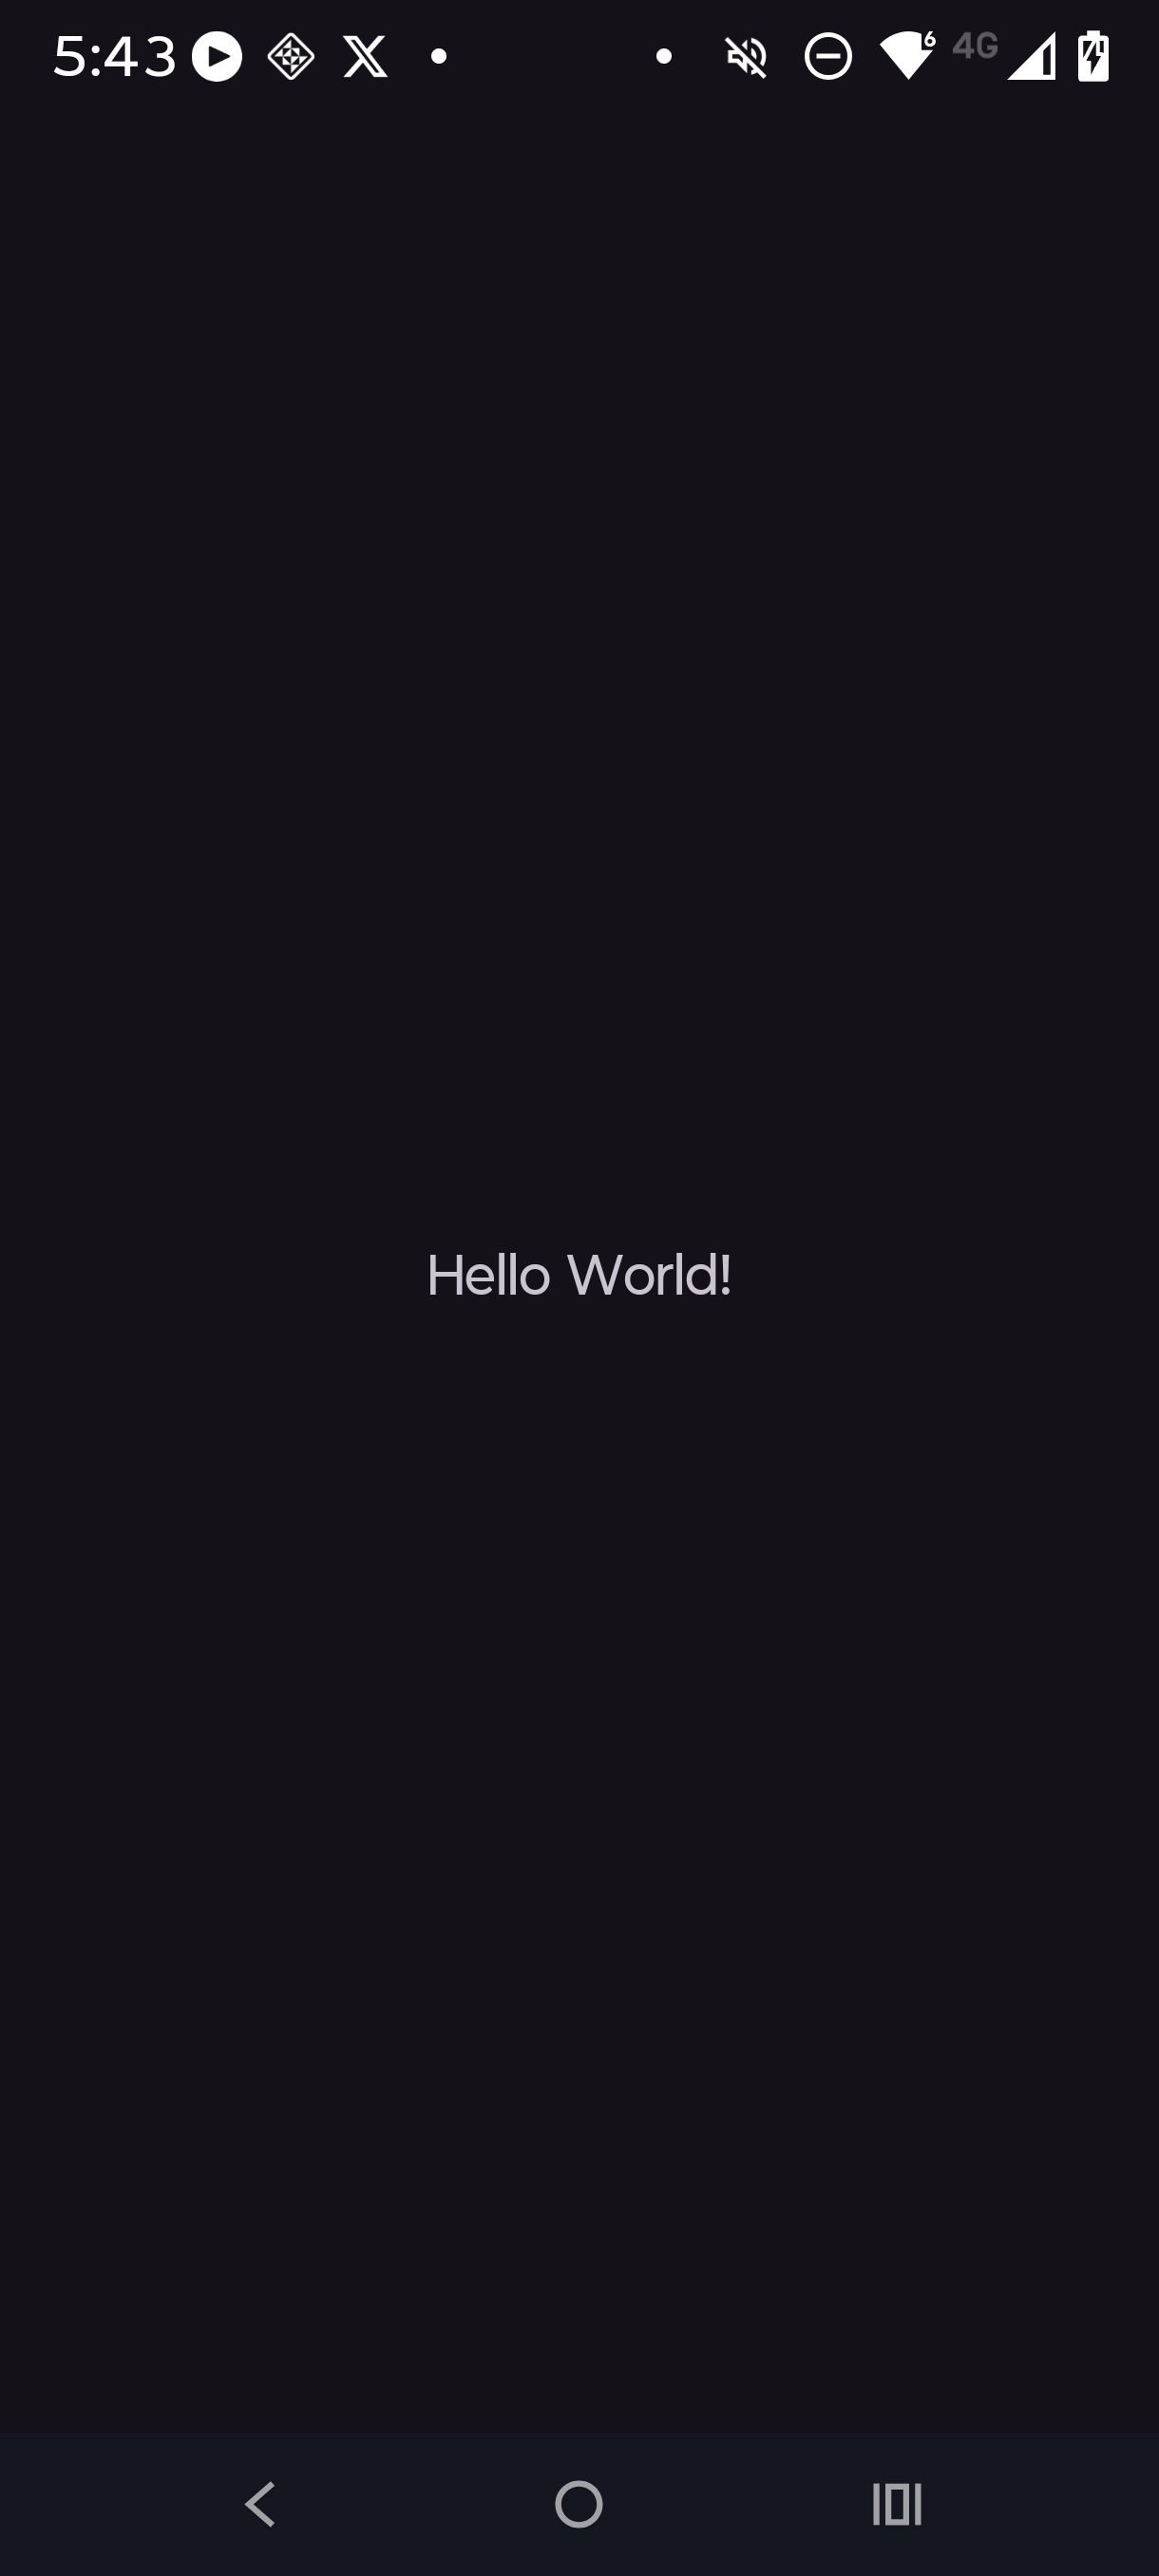
\includegraphics[width=0.98\textwidth]{02_TallerCBTis/figs/Demo00}
\end{center}
\end{column}
\end{columns}

\end{frame}


\begin{frame}[fragile]
\frametitle{Demo 01: Modificar el activity\_main.xml para aregar otro TextView}
\begin{columns}
\column{0.80\linewidth}
De los códigos fuentes en Github (como un archivo .zip), descomprimirlo y localizar los archivos mencionados a continuación:
\begin{itemize}
\item Copiar el archivo \textit{MainActivity\_Demo01.java} (dentro del Folder códigosJAVA) al mismo directorio donde esta el \textit{MainActivity.java}.
\item Copiar el archivo \textit{activity\_main\_demo01.xml} (dentro del Folder Carpeta\_layout) al mismo directorio donde esta el \textit{activity\_main.xml}
\item Modificar en el archivo AndroidManifest.xml la cadena \textit{.MainActivity} por \textit{.MainActivity\_Demo01}.
\end{itemize}

\begin{block}{Demo \#01}
Muestra un TextView con el texto centrado "Hello World!" (fuente verde, fondo rojo) 
\end{block}


\column{0.20\linewidth}

\begin{center}
 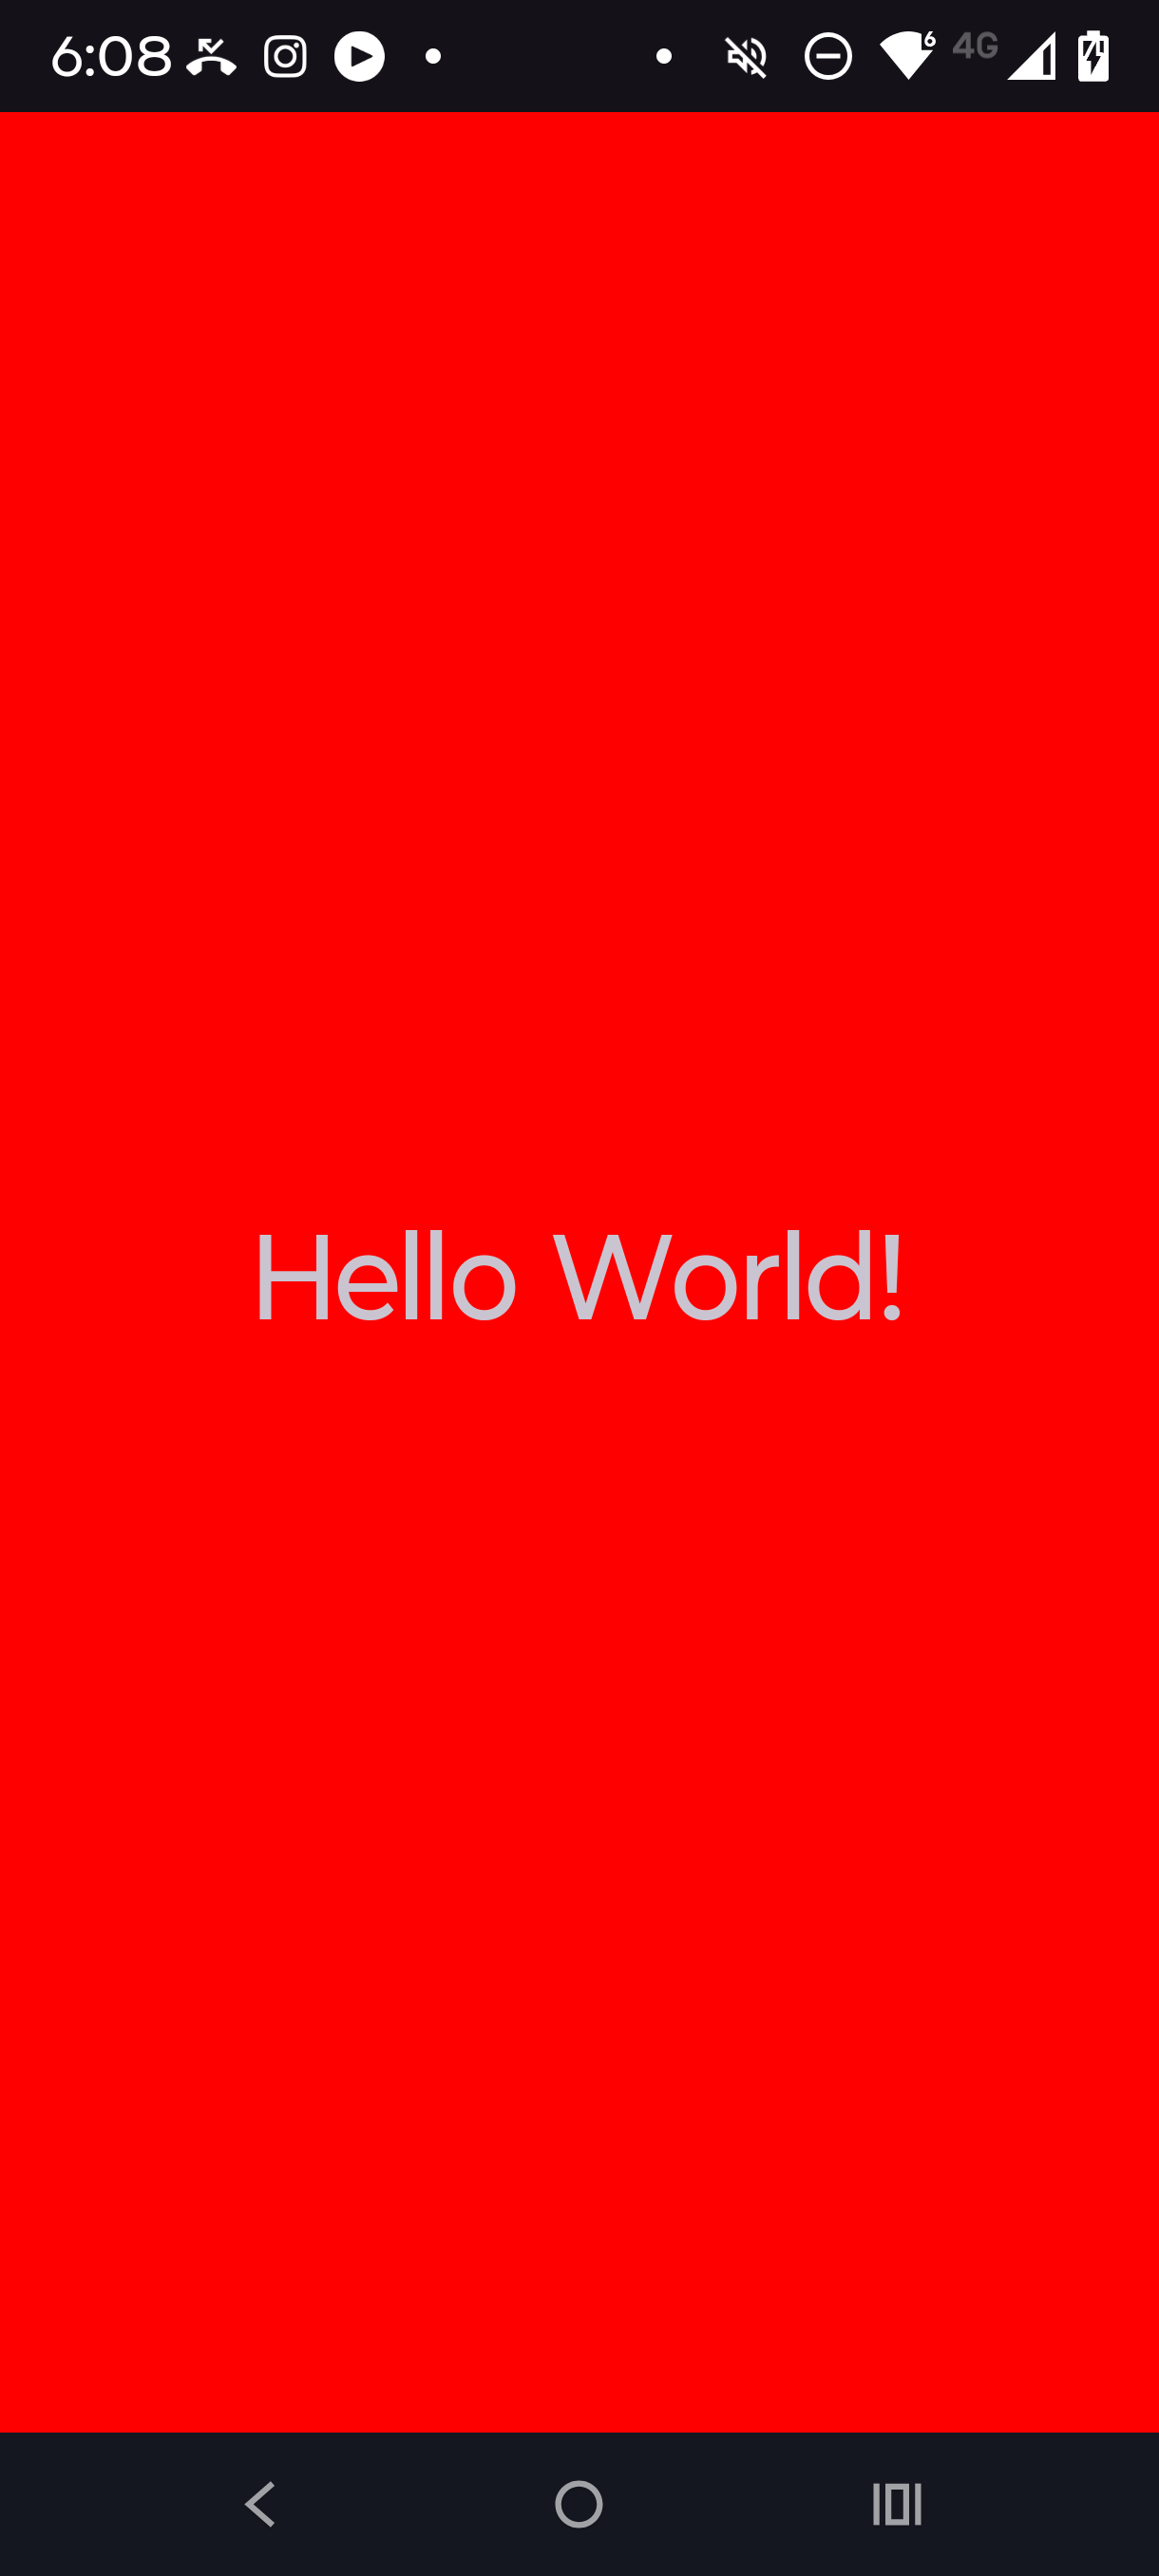
\includegraphics[width=0.98\textwidth]{02_TallerCBTis/figs/Demo01}
\end{center}

\end{columns}

\end{frame}


\begin{frame}{Modificaciones de Interés}

\begin{block}{Ejercicio \#01}
\begin{itemize}
\item Duplicar el TextView pero modificando el color de dichos componentes. 
\item Probar diferentes combinaciones del valor \textit{layout\_weight} en dichos componentes. 

\end{itemize}
\end{block}


\end{frame}

\begin{frame}{Componentes EditText y Button en Android}

\textbf{EditText: Campo de Entrada de Texto}
\begin{itemize}
    \item Permite al usuario introducir y editar texto dentro de la aplicación.
    \item Se utiliza en formularios, búsquedas y captura de datos.
    \item Soporta distintos tipos de entrada (texto, número, correo, contraseña).
    \item Puede configurarse mediante atributos XML o código Java/Kotlin.
\end{itemize}

\vspace{0.4cm}

\textbf{Button: Botón de Interacción}
\begin{itemize}
    \item Es un componente que permite al usuario ejecutar acciones al hacer clic.
    \item Se utiliza para enviar datos, navegar entre pantallas o activar eventos.
    \item Puede personalizarse en texto, color, tamaño y estilo.
\end{itemize}


\end{frame}



\begin{frame}[fragile]
\frametitle{Demo 02: Agregar un EditText y un Button}
\begin{columns}
\column{0.80\linewidth}
De los códigos fuentes en Github (como un archivo .zip), descomprimirlo y localizar los archivos mencionados a continuación:
\begin{itemize}
\item Copiar el archivo \textit{MainActivity\_Demo02.java} (dentro del Folder códigosJAVA) al mismo directorio donde esta el \textit{MainActivity.java}.
\item Copiar el archivo \textit{activity\_main\_demo02.xml} (dentro del Folder Carpeta\_layout) al mismo directorio donde esta el \textit{activity\_main.xml}.
\item Modificar en el archivo \textit{AndroidManifest.xml} la cadena \textit{..MainActivity\_Demo01} por \textit{.MainActivity\_Demo02}
\end{itemize}

\begin{block}{Demo \#02}
Muestra una App con dos TextViews, un EditText y un Botton. Cuando el usuario ingresa un dato y presiona le boton aparece un mensaje con el dato ingresado 
\end{block}


\column{0.20\linewidth}

\begin{center}
 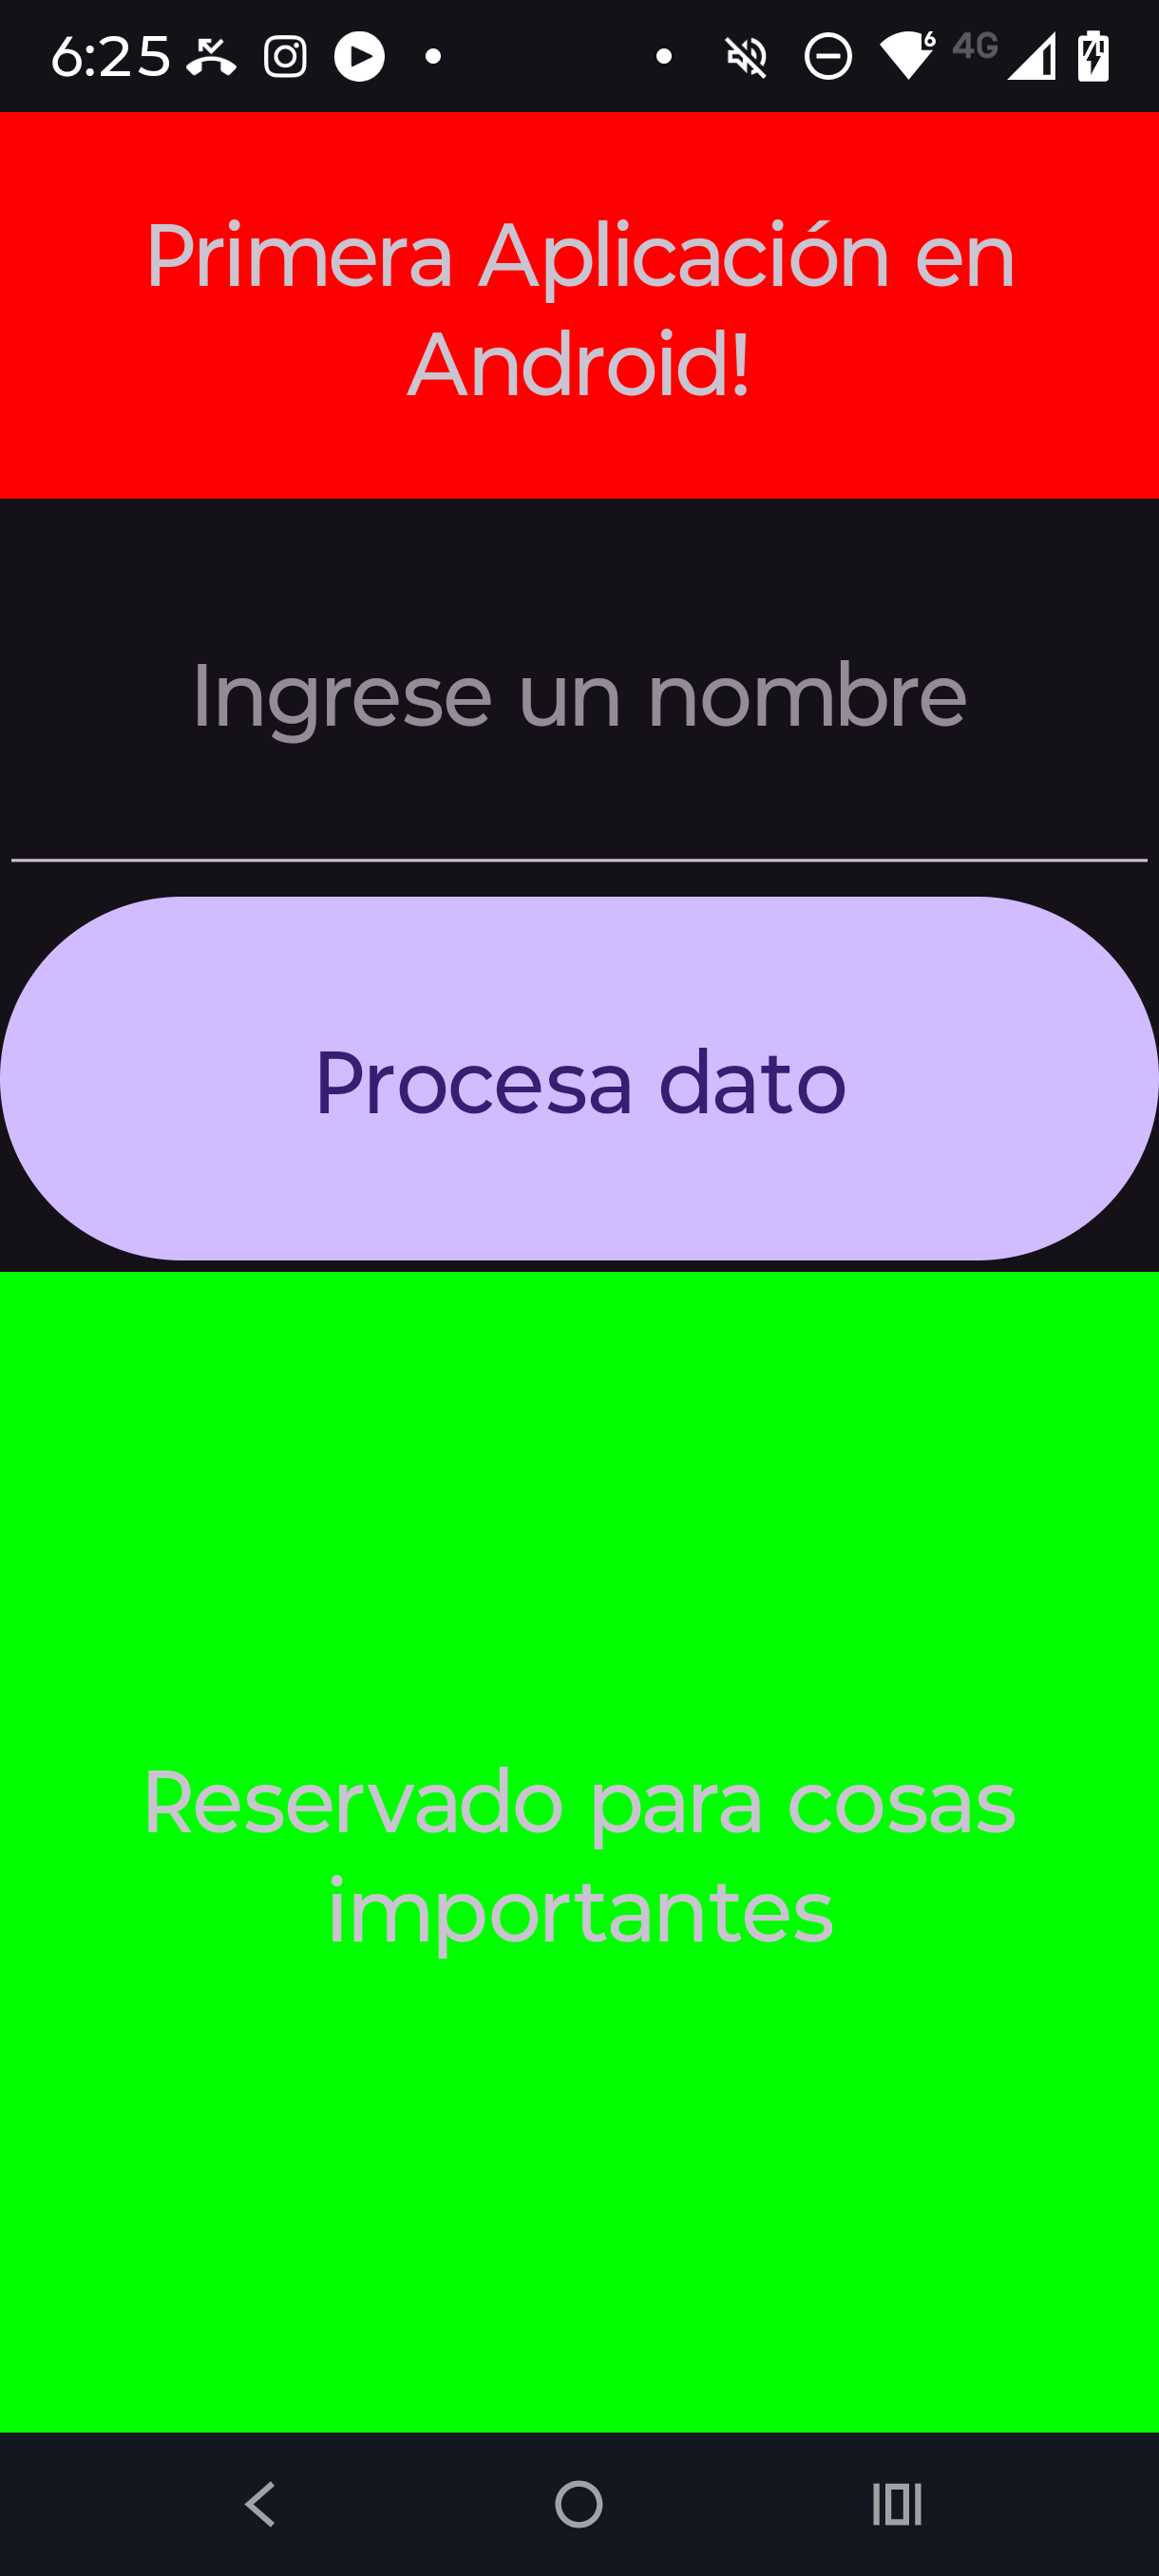
\includegraphics[width=0.98\textwidth]{02_TallerCBTis/figs/Demo02}
\end{center}

\end{columns}

\end{frame}


\begin{frame}{Uso de GridLayout en Android}
\textbf{¿Qué es GridLayout?}

\begin{itemize}
    \item Es un contenedor de diseño (ViewGroup) que organiza los elementos en una cuadrícula de filas y columnas.
    \item Permite ubicar componentes de manera estructurada y alineada.
\end{itemize}

\vspace{0.4cm}

\textbf{¿Para qué sirve?}
\begin{itemize}
    \item Diseñar interfaces organizadas en forma de tabla.
    \item Alinear múltiples elementos (botones, imágenes, textos) fácilmente.
    \item Crear interfaces dinámicas como teclados, galerías o tableros de juego.
\end{itemize}

\vspace{0.4cm}

\textbf{Características principales:}
\begin{itemize}
    \item Define número de filas y columnas.
    \item Permite que los elementos ocupen múltiples celdas (rowSpan, columnSpan).
    \item Soporta alineación y distribución del espacio.
\end{itemize}


\end{frame}


\begin{frame}[fragile]
\frametitle{Demo 03: Agregar un Panel de Botones utilizando un GridLayout}
\begin{columns}
\column{0.80\linewidth}
Del Repositorio Github:
\begin{itemize}
\item Copiar el archivo MainActivity\_Demo03.java (dentro del Folder códigosJAVA) al mismo directorio donde esta el MainActivity.java
\item Copiar el archivo activity\_main\_demo03.xml (dentro del Folder Carpeta\_layout) al mismo directorio donde esta el activity\_main.xml
\item Modificar en el archivo AndroidManifest.xml la cadena \textit{.MainActivity\_Demo02} por \textit{.MainActivity\_Demo03}
\end{itemize}

\begin{block}{Demo \#03}
Muestra una App con un panel de botones, que muestra un Toast para cada boton presionado por el usuario.  
\end{block}


\column{0.20\linewidth}

\begin{center}
 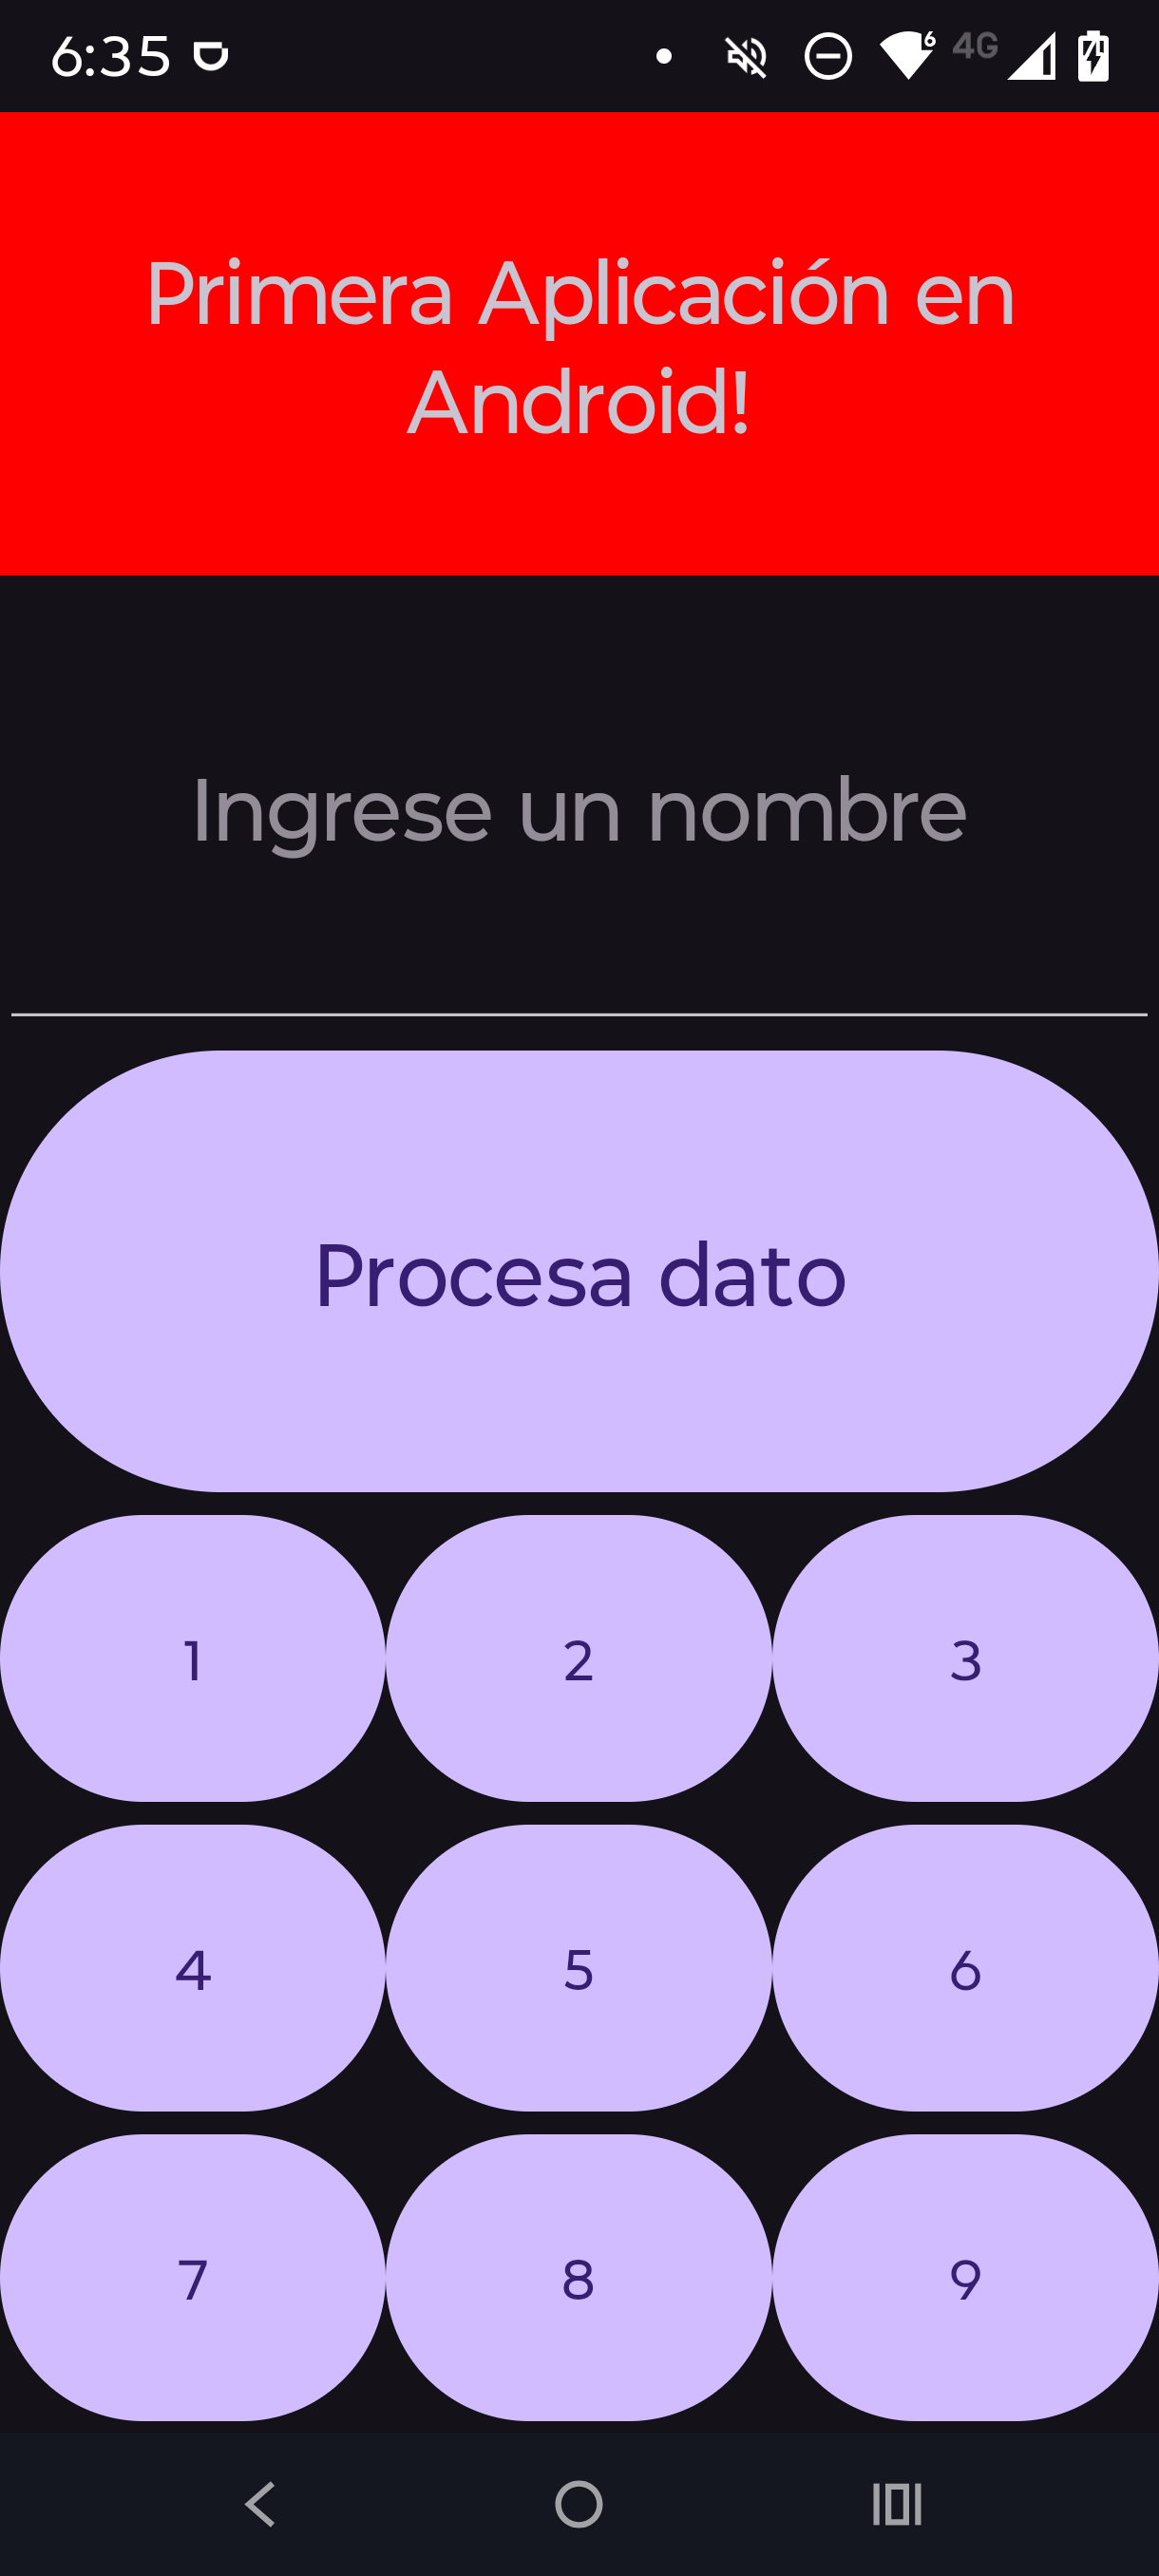
\includegraphics[width=0.98\textwidth]{02_TallerCBTis/figs/Demo03}
\end{center}

\end{columns}

\end{frame}



\begin{frame}{Componentes CheckBox e ImageView en Android}

\textbf{CheckBox: ¿Para qué sirve?}
\begin{itemize}
    \item Permite al usuario seleccionar una o múltiples opciones de una lista.
    \item Cada opción es independiente (no excluyente).
    \item Es útil en formularios, configuraciones o encuestas.
\end{itemize}

\vspace{0.4cm}

\textbf{Características del CheckBox:}
\begin{itemize}
    \item Puede estar en estado seleccionado o no seleccionado.
    \item Permite manejar eventos de cambio (OnCheckedChangeListener).
\end{itemize}

\vspace{0.4cm}

\textbf{ImageView: ¿Para qué sirve?}
\begin{itemize}
    \item Se utiliza para mostrar imágenes en la interfaz de usuario.
    \item Soporta recursos locales (drawable) o imágenes desde URL.
\end{itemize}

\vspace{0.4cm}

\textbf{Características del ImageView:}
\begin{itemize}
    \item Permite escalar, ajustar y posicionar imágenes.
    \item Compatible con diferentes formatos (PNG, JPG, SVG - mediante librerías).
\end{itemize}


\end{frame}


\begin{frame}[fragile]
\frametitle{Demo 04: Agregar un CheckBox y un ImageView}
\begin{columns}
\column{0.80\linewidth}
Del Repositorio Github:
\begin{itemize}
\item Copiar el archivo MainActivity\_Demo04.java (dentro del Folder códigosJAVA) al mismo directorio donde esta el MainActivity.java
\item Copiar el archivo activity\_main\_demo04.xml (dentro del Folder Carpeta\_layout) al mismo directorio donde esta el activity\_main.xml
\item Copiar el archivo \textit{upv.png} dentro de la folder \textit{Carpeta\_drawable} en el directorio \textit{res/drawable} del proyecto de AS.


\item Modificar en el archivo AndroidManifest.xml la cadena \textit{.MainActivity\_Demo03} por \textit{.MainActivity\_Demo04}
\end{itemize}

\begin{block}{Demo \#04}
Una App con in Checkbox y un ImageView. Al modificar el estado del CheckBox, el texto de un Textview cambia. Al presionar el primer boton, un Toast muestra el estado del Checkbox.  
\end{block}


\column{0.20\linewidth}

\begin{center}
 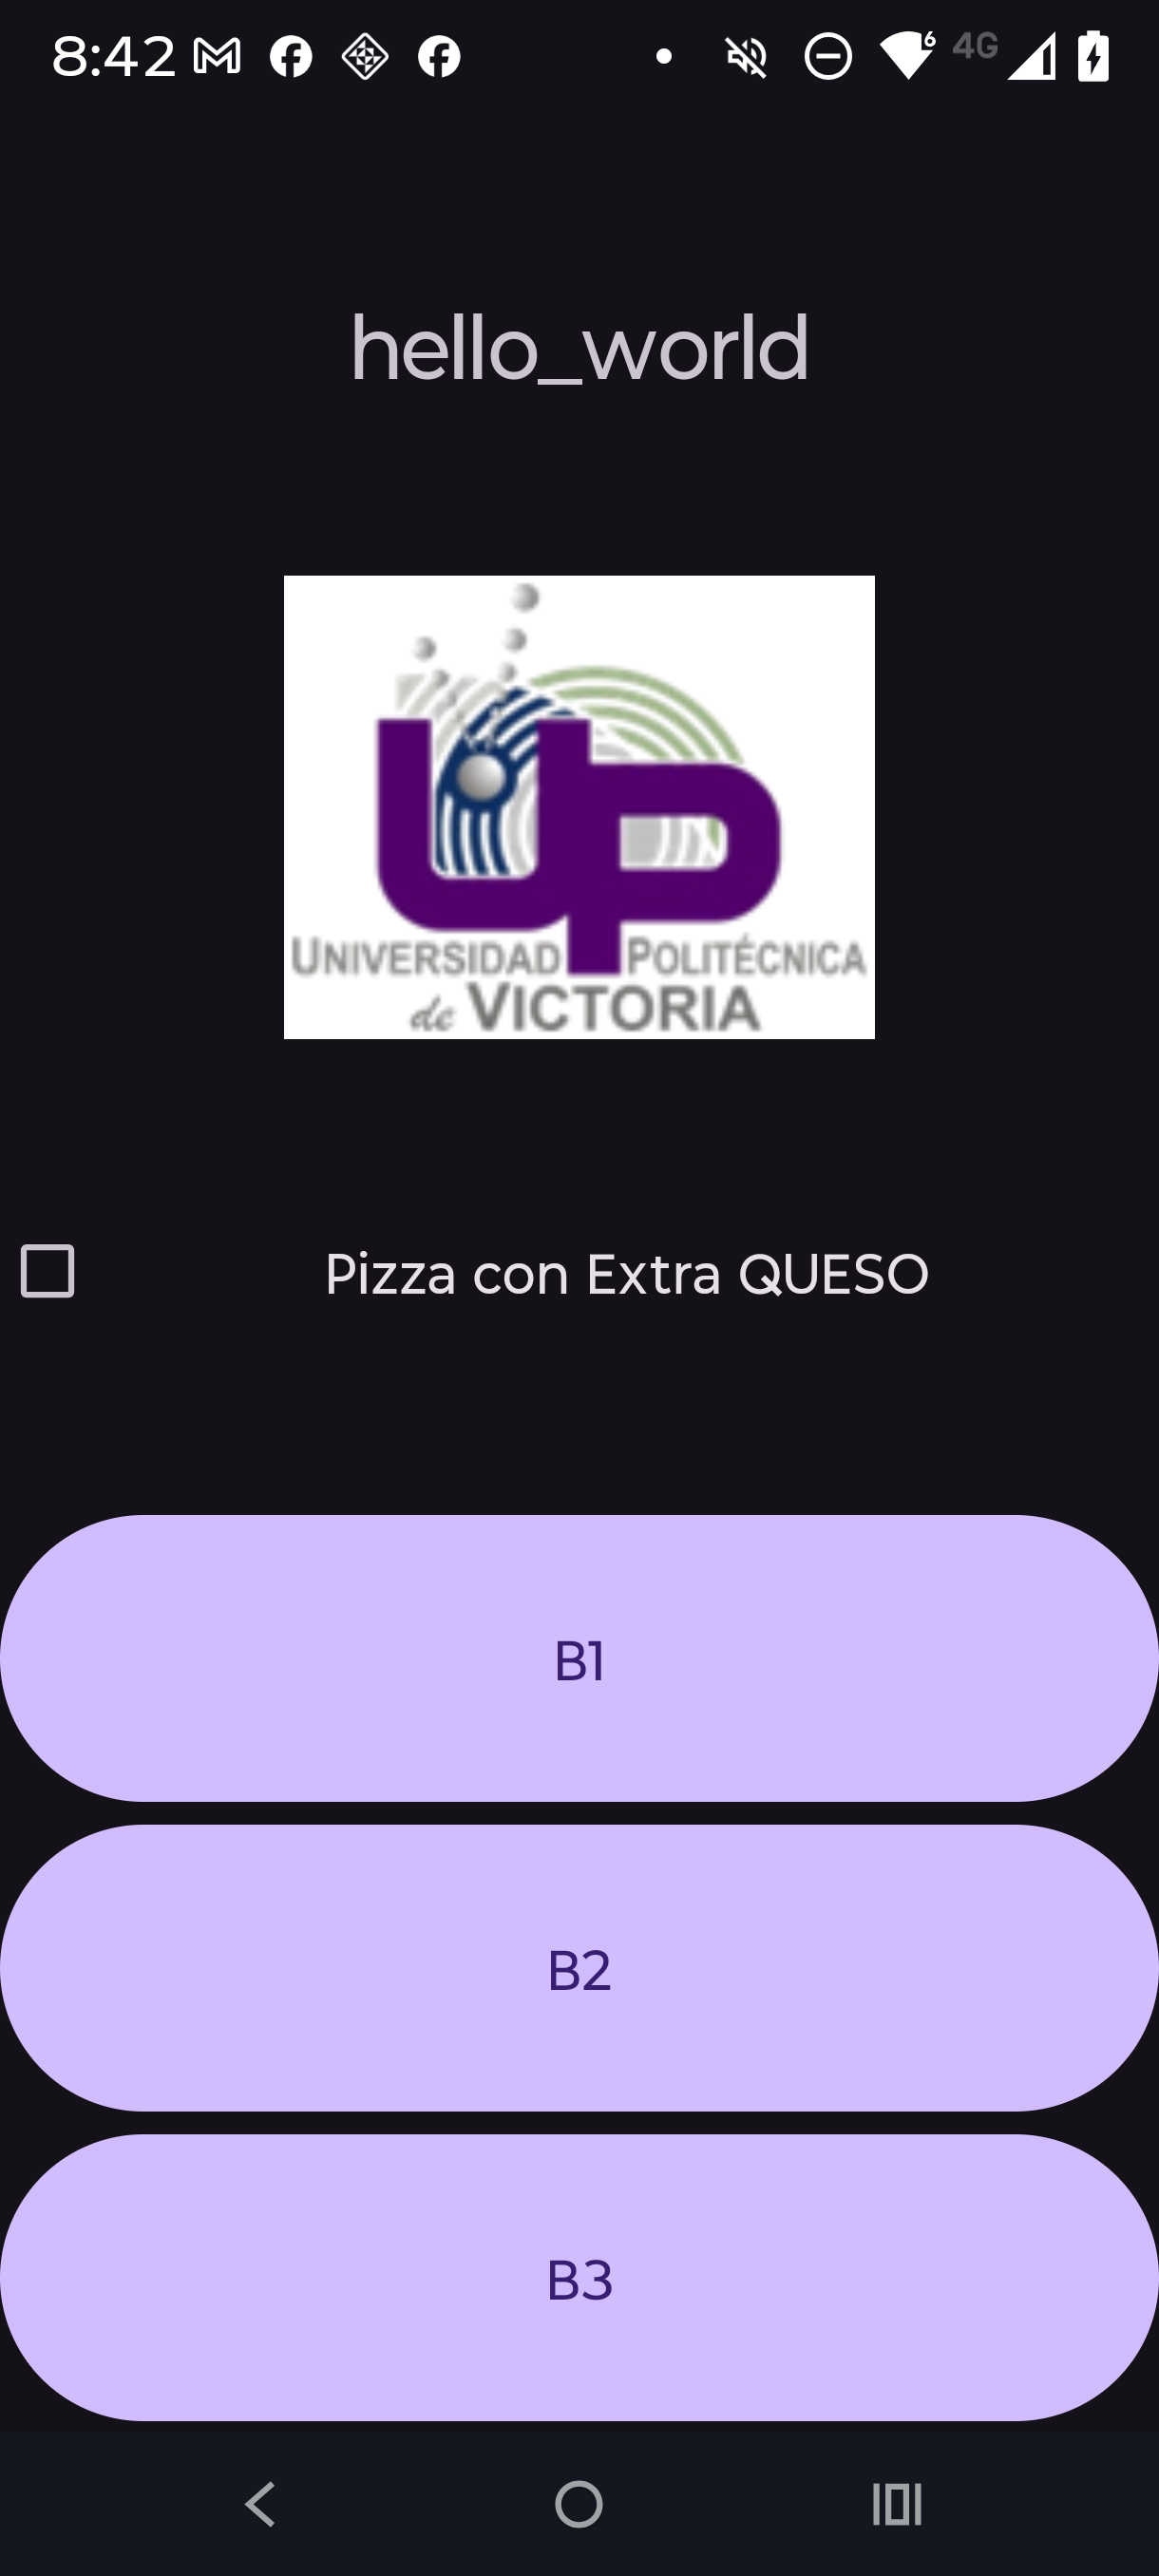
\includegraphics[width=0.98\textwidth]{02_TallerCBTis/figs/Demo04}
\end{center}

\end{columns}

\end{frame}


\begin{frame}[fragile]
\frametitle{Demo 05: Agregar un RadioGroup}
\begin{columns}
\column{0.80\linewidth}
Del Repositorio Github:
\begin{itemize}
\item Copiar el archivo MainActivity\_Demo05.java (dentro del Folder códigosJAVA) al mismo directorio donde esta el MainActivity.java
\item Copiar el archivo activity\_main\_demo05.xml (dentro del Folder Carpeta\_layout) al mismo directorio donde esta el activity\_main.xml
\item Copiar los archivos \textit{cgup.jpg} y \textit{logo\_upv\_2019.png} localizados dentro de la folder \textit{Carpeta\_drawable} en el directorio \textit{res/drawable} del proyecto de AS.
\item Modificar en el archivo AndroidManifest.xml la cadena \textit{.MainActivity\_Demo04} por \textit{.MainActivity\_Demo05}
\end{itemize}

\begin{block}{Demo \#05}
Muestra una App con un RadioGroup. El ImageView cambia basado en la seleccion del usuario.    
\end{block}


\column{0.20\linewidth}

\begin{center}
 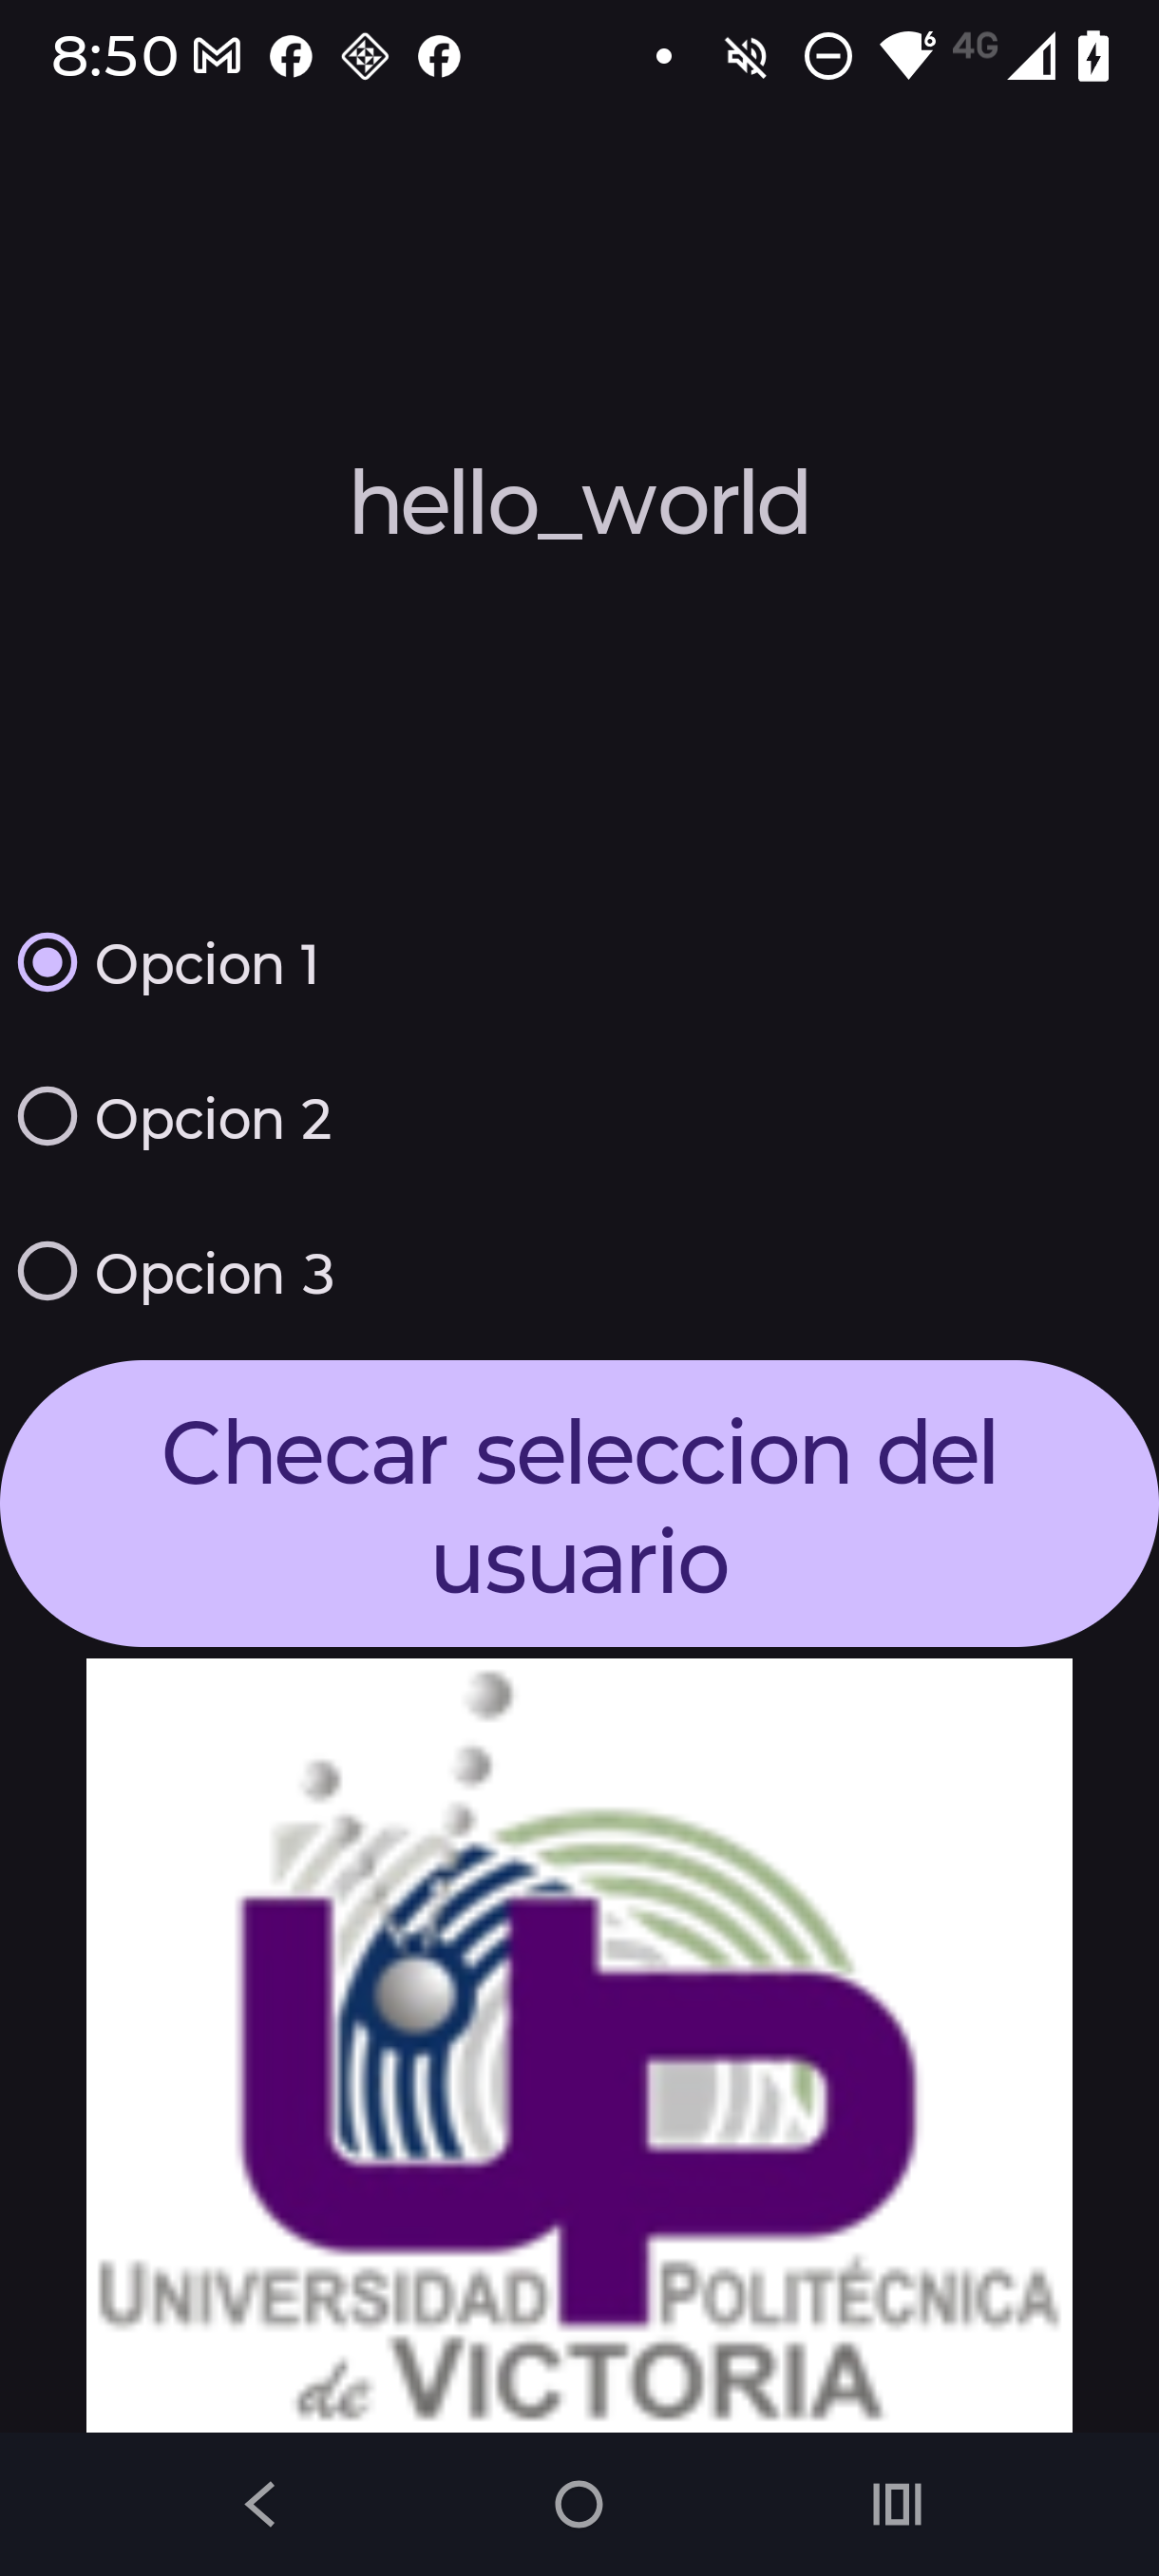
\includegraphics[width=0.98\textwidth]{02_TallerCBTis/figs/Demo05}
\end{center}

\end{columns}

\end{frame}

\begin{frame}{Componentes Adapter y ListView en Android}
\textbf{¿Qué es ListView?}

\begin{itemize}
    \item Es un componente de interfaz que permite mostrar una lista desplazable de elementos.
    \item Cada elemento puede contener texto, imágenes u otros componentes.
    \item Es útil para mostrar datos en forma de lista vertical.
\end{itemize}

\vspace{0.4cm}

\textbf{¿Qué es un Adapter?}

\begin{itemize}
    \item Es un intermediario entre los datos y el ListView.
    \item Se encarga de convertir los datos (arreglos, listas, bases de datos) en vistas visuales.
    \item Permite personalizar cómo se muestra cada elemento de la lista.
\end{itemize}

\vspace{0.4cm}

\textbf{Relación entre Adapter y ListView:}
\begin{itemize}
    \item El ListView solicita los datos al Adapter.
    \item El Adapter genera la vista de cada elemento.
\end{itemize}


\end{frame}



\begin{frame}[fragile]
\frametitle{Demo 06: Agregar un ListView}
\begin{columns}
\column{0.80\linewidth}
Del Repositorio Github:
\begin{itemize}
\item Copiar el archivo MainActivity\_Demo06.java (dentro del Folder códigosJAVA) al mismo directorio donde esta el MainActivity.java
\item Copiar el archivo activity\_main\_demo06.xml (dentro del Folder Carpeta\_layout) al mismo directorio donde esta el activity\_main.xml
%\item Copiar los archivos \textit{cgup.jpg} y \textit{logo\_upv\_2019.png} localizados dentro de la folder \textit{Carpeta\_drawable} en el directorio \textit{res/drawable} del proyecto de AS.
\item Modificar en el archivo AndroidManifest.xml la cadena \textit{.MainActivity\_Demo05} por \textit{.MainActivity\_Demo06}
\end{itemize}

\begin{block}{Demo \#06}
Muestra una App con un ListView. El usuario agregar elementos al presionar el boton superior.    
\end{block}


\column{0.20\linewidth}

\begin{center}
 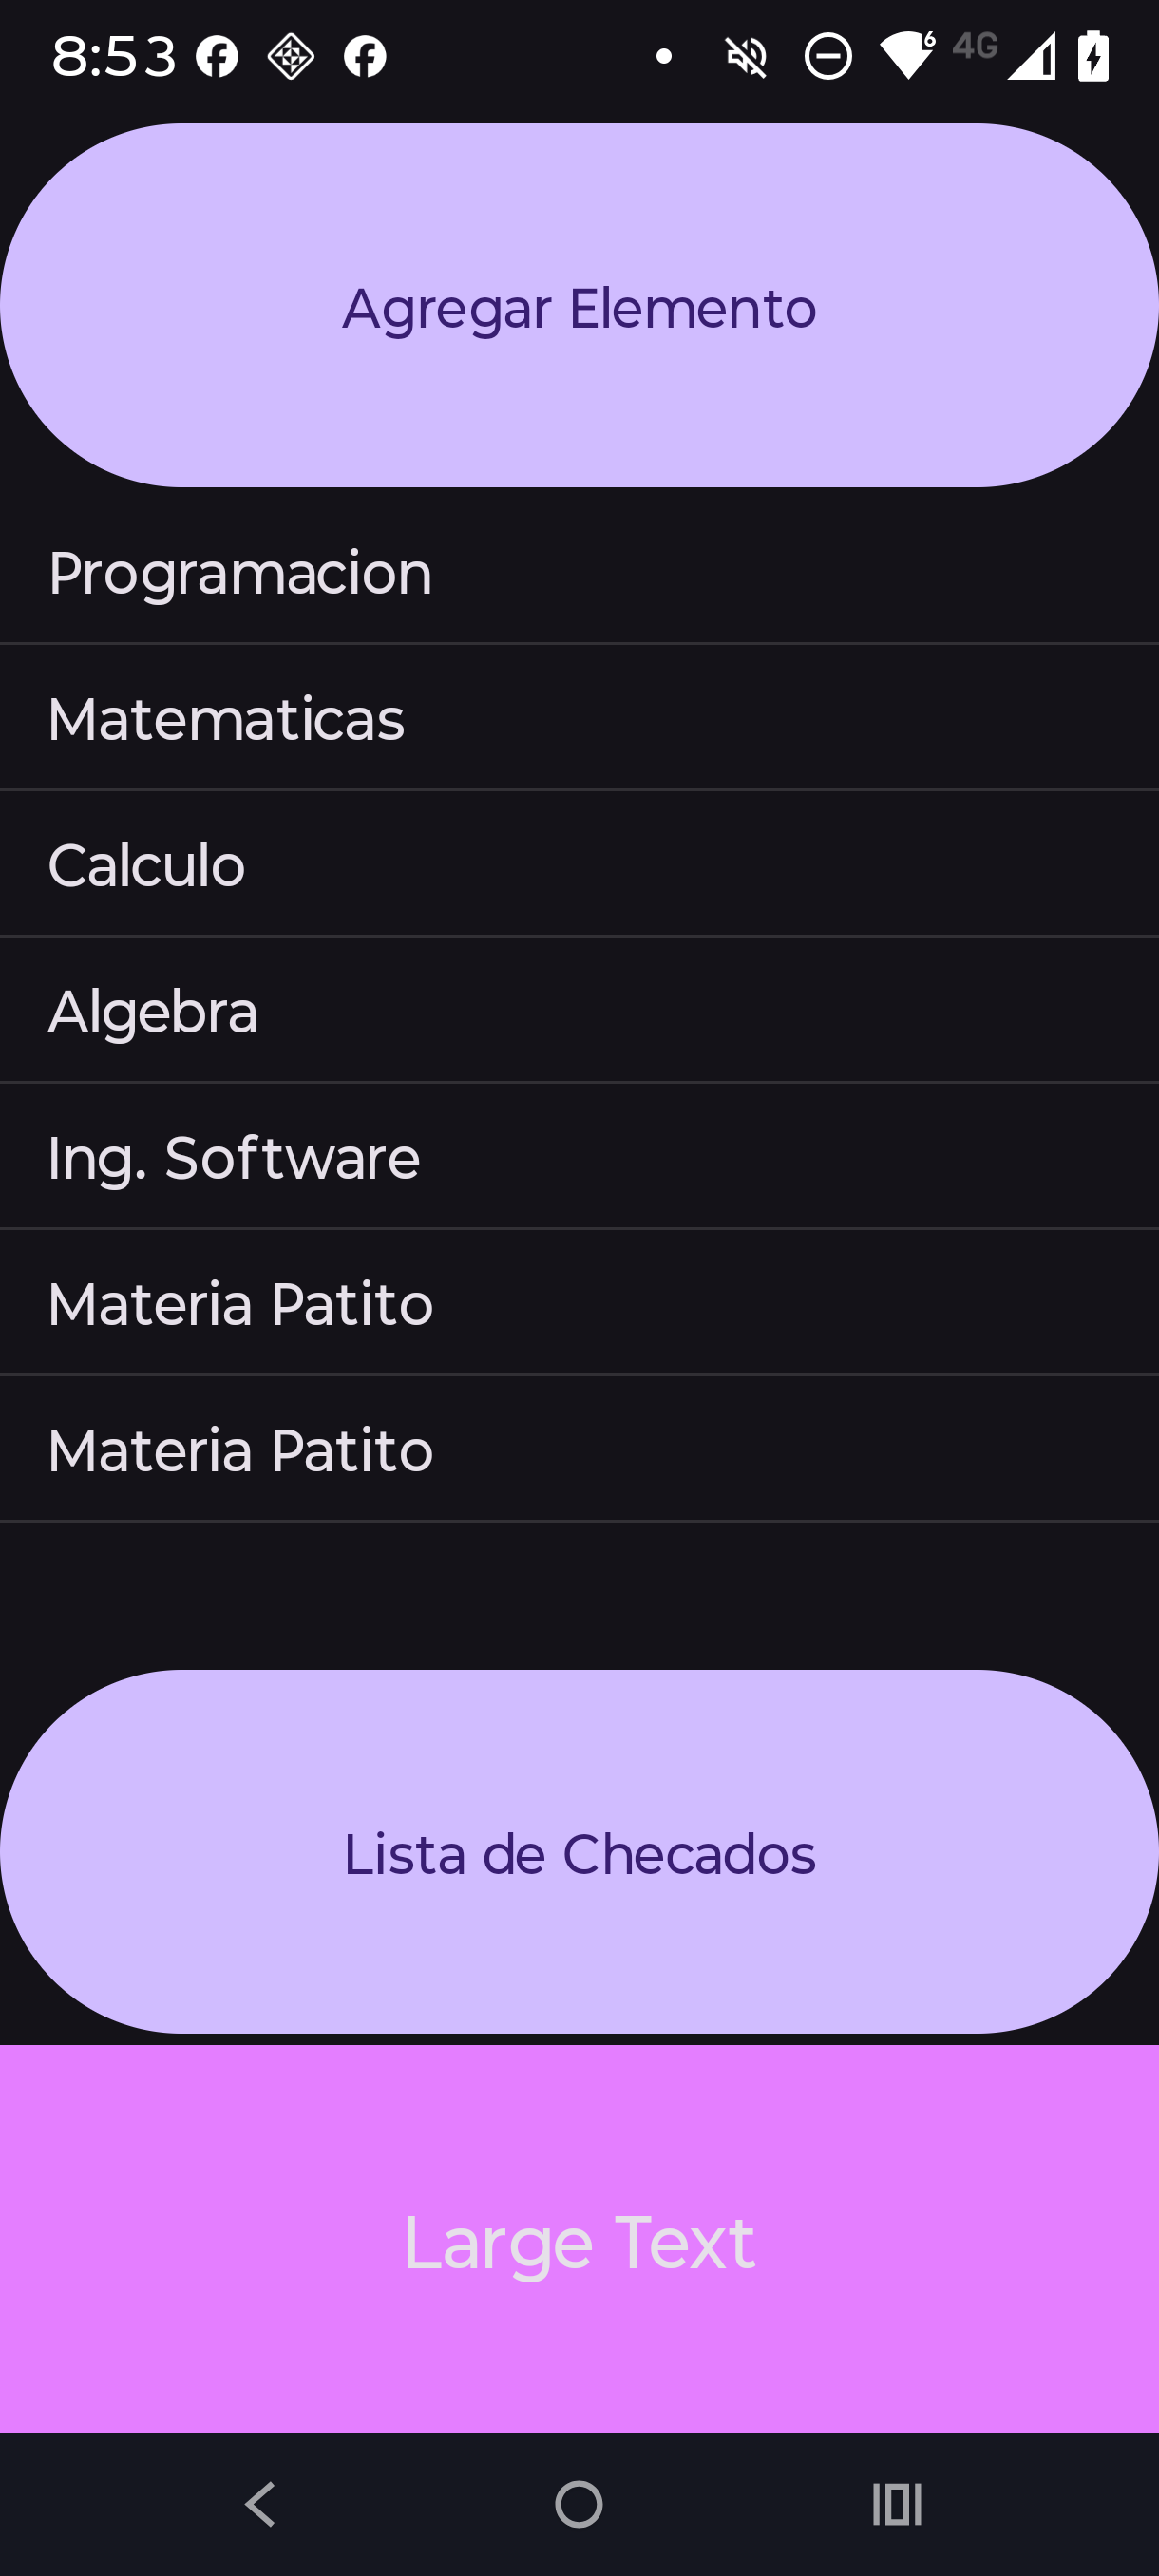
\includegraphics[width=0.98\textwidth]{02_TallerCBTis/figs/Demo06}
\end{center}

\end{columns}

\end{frame}


\begin{frame}{Spinner vs ListView en Android}
\textbf{¿Qué es un Spinner?}

\begin{itemize}
    \item Es un componente que permite seleccionar una opción de una lista desplegable.
    \item Ocupa poco espacio en pantalla.
    \item Ideal cuando se requiere elegir una sola opción entre varias.
\end{itemize}

\vspace{0.4cm}

\textbf{¿Qué es un ListView?}

\begin{itemize}
    \item Es un componente que muestra una lista de elementos visibles en pantalla.
    \item Permite visualizar múltiples opciones al mismo tiempo.
    \item Puede soportar selección simple o múltiple.
\end{itemize}

\vspace{0.4cm}

\textbf{Diferencias principales:}

\begin{itemize}
    \item \textbf{Espacio:} Spinner es compacto, ListView requiere más espacio.
    \item \textbf{Interacción:} Spinner usa menú desplegable, ListView muestra lista directa.
    \item \textbf{Uso:} Spinner para selección rápida; ListView para exploración de datos.
    \item \textbf{Cantidad de datos:} ListView es más adecuado para listas largas.
\end{itemize}

\end{frame}



\begin{frame}[fragile]
\frametitle{Demo 07: Agregar un Spinner}
\begin{columns}
\column{0.80\linewidth}
Del Repositorio Github:
\begin{itemize}
\item Copiar el archivo MainActivity\_Demo07.java (dentro del Folder códigosJAVA) al mismo directorio donde esta el MainActivity.java
\item Copiar el archivo activity\_main\_demo07.xml (dentro del Folder Carpeta\_layout) al mismo directorio donde esta el activity\_main.xml
%\item Copiar los archivos \textit{cgup.jpg} y \textit{logo\_upv\_2019.png} localizados dentro de la folder \textit{Carpeta\_drawable} en el directorio \textit{res/drawable} del proyecto de AS.
\item Modificar en el archivo AndroidManifest.xml la cadena \textit{.MainActivity\_Demo06} por \textit{.MainActivity\_Demo07}
\end{itemize}

\begin{block}{Demo \#07}
Muestra una App con un ListView. El usuario agregar elementos al presionar el boton superior.    
\end{block}


\column{0.20\linewidth}

\begin{center}
 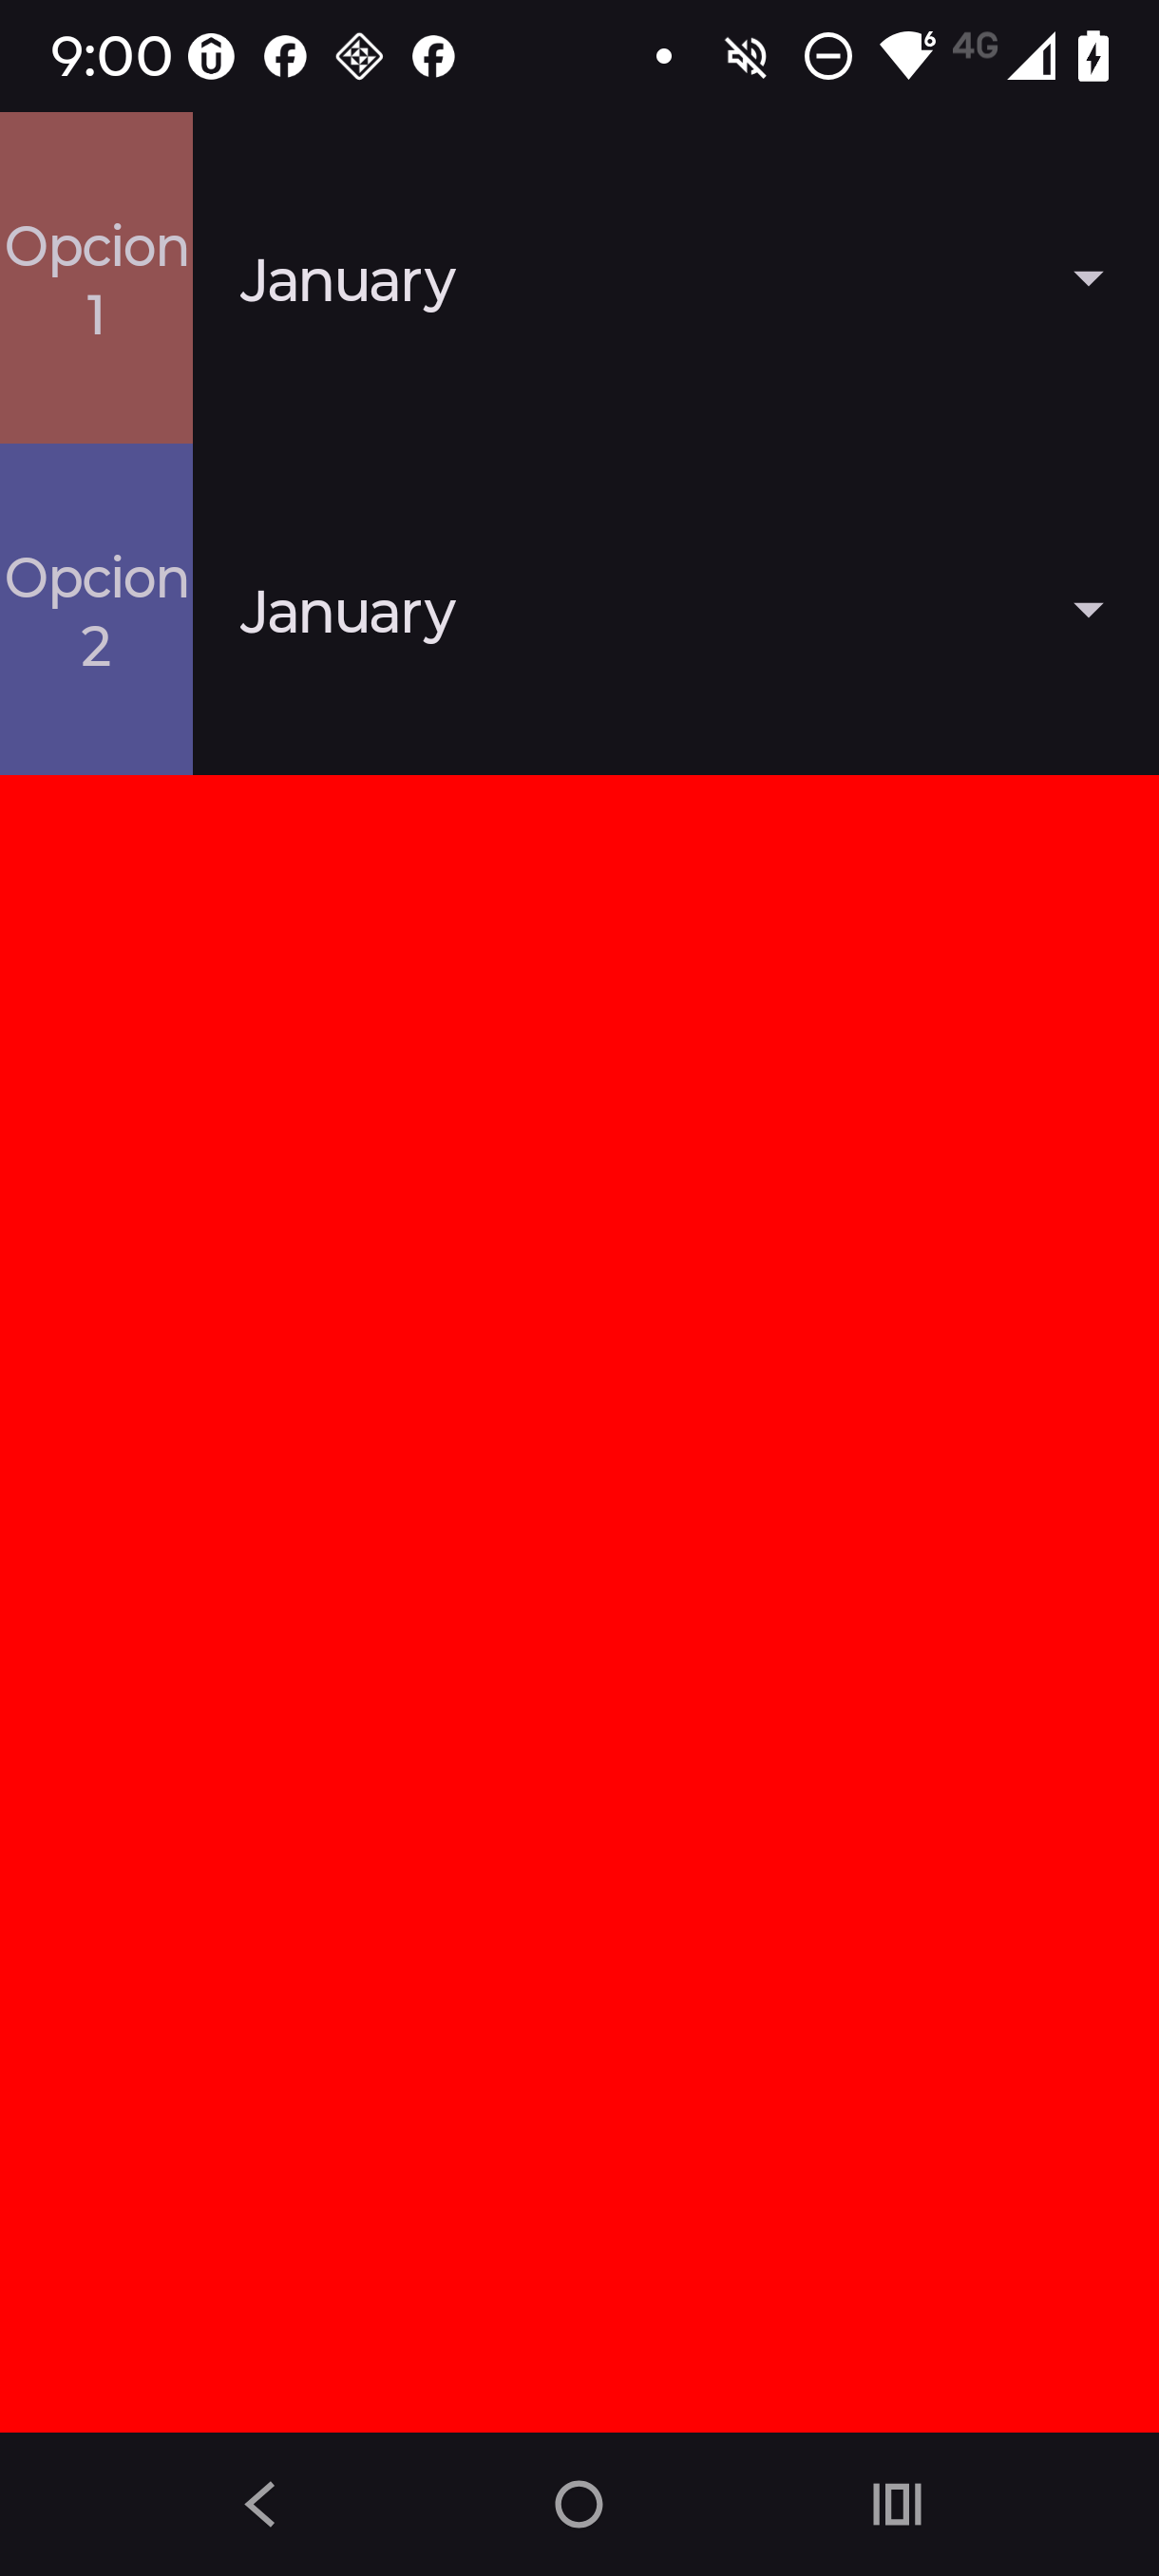
\includegraphics[width=0.98\textwidth]{02_TallerCBTis/figs/Demo07}
\end{center}

\end{columns}

\end{frame}


\begin{frame}{Componente SeekBar en Android}
\textbf{¿Qué es un SeekBar?}

\begin{itemize}
    \item Es un componente de interfaz gráfica que permite al usuario seleccionar un valor dentro de un rango deslizando un control horizontal.
    \item Es una extensión de la clase ProgressBar con interacción del usuario.
\end{itemize}

\vspace{0.5cm}

\textbf{¿Para qué sirve?}
\begin{itemize}
    \item Ajustar valores continuos o discretos (ej. volumen, brillo, progreso).
    \item Permitir entrada intuitiva mediante deslizamiento.
    \item Controlar parámetros en tiempo real.
\end{itemize}

\vspace{0.5cm}

\textbf{Características principales:}
\begin{itemize}
    \item Permite definir valores mínimo, máximo y progreso actual.
    \item Puede escuchar cambios mediante un listener (OnSeekBarChangeListener).
    \item Es altamente personalizable (colores, tamaño, estilo).
\end{itemize}


\end{frame}


\begin{frame}[fragile]
\frametitle{Demo 08: Agregar SeekBars}
\begin{columns}
\column{0.80\linewidth}
Del Repositorio Github:
\begin{itemize}
\item Copiar el archivo MainActivity\_Demo08.java (dentro del Folder códigosJAVA) al mismo directorio donde esta el MainActivity.java
\item Copiar el archivo activity\_main\_demo08.xml (dentro del Folder Carpeta\_layout) al mismo directorio donde esta el activity\_main.xml
%\item Copiar los archivos \textit{cgup.jpg} y \textit{logo\_upv\_2019.png} localizados dentro de la folder \textit{Carpeta\_drawable} en el directorio \textit{res/drawable} del proyecto de AS.
\item Modificar en el archivo AndroidManifest.xml la cadena \textit{.MainActivity\_Demo07} por \textit{.MainActivity\_Demo08}
\end{itemize}

\begin{block}{Demo \#08}
Muestra una App dos SeekBars (la segunda utiliza separadores finitos). La primera SeekBar actualiza el contenido de TextView conforme la seleccion del usuario. 
\end{block}


\column{0.20\linewidth}

\begin{center}
 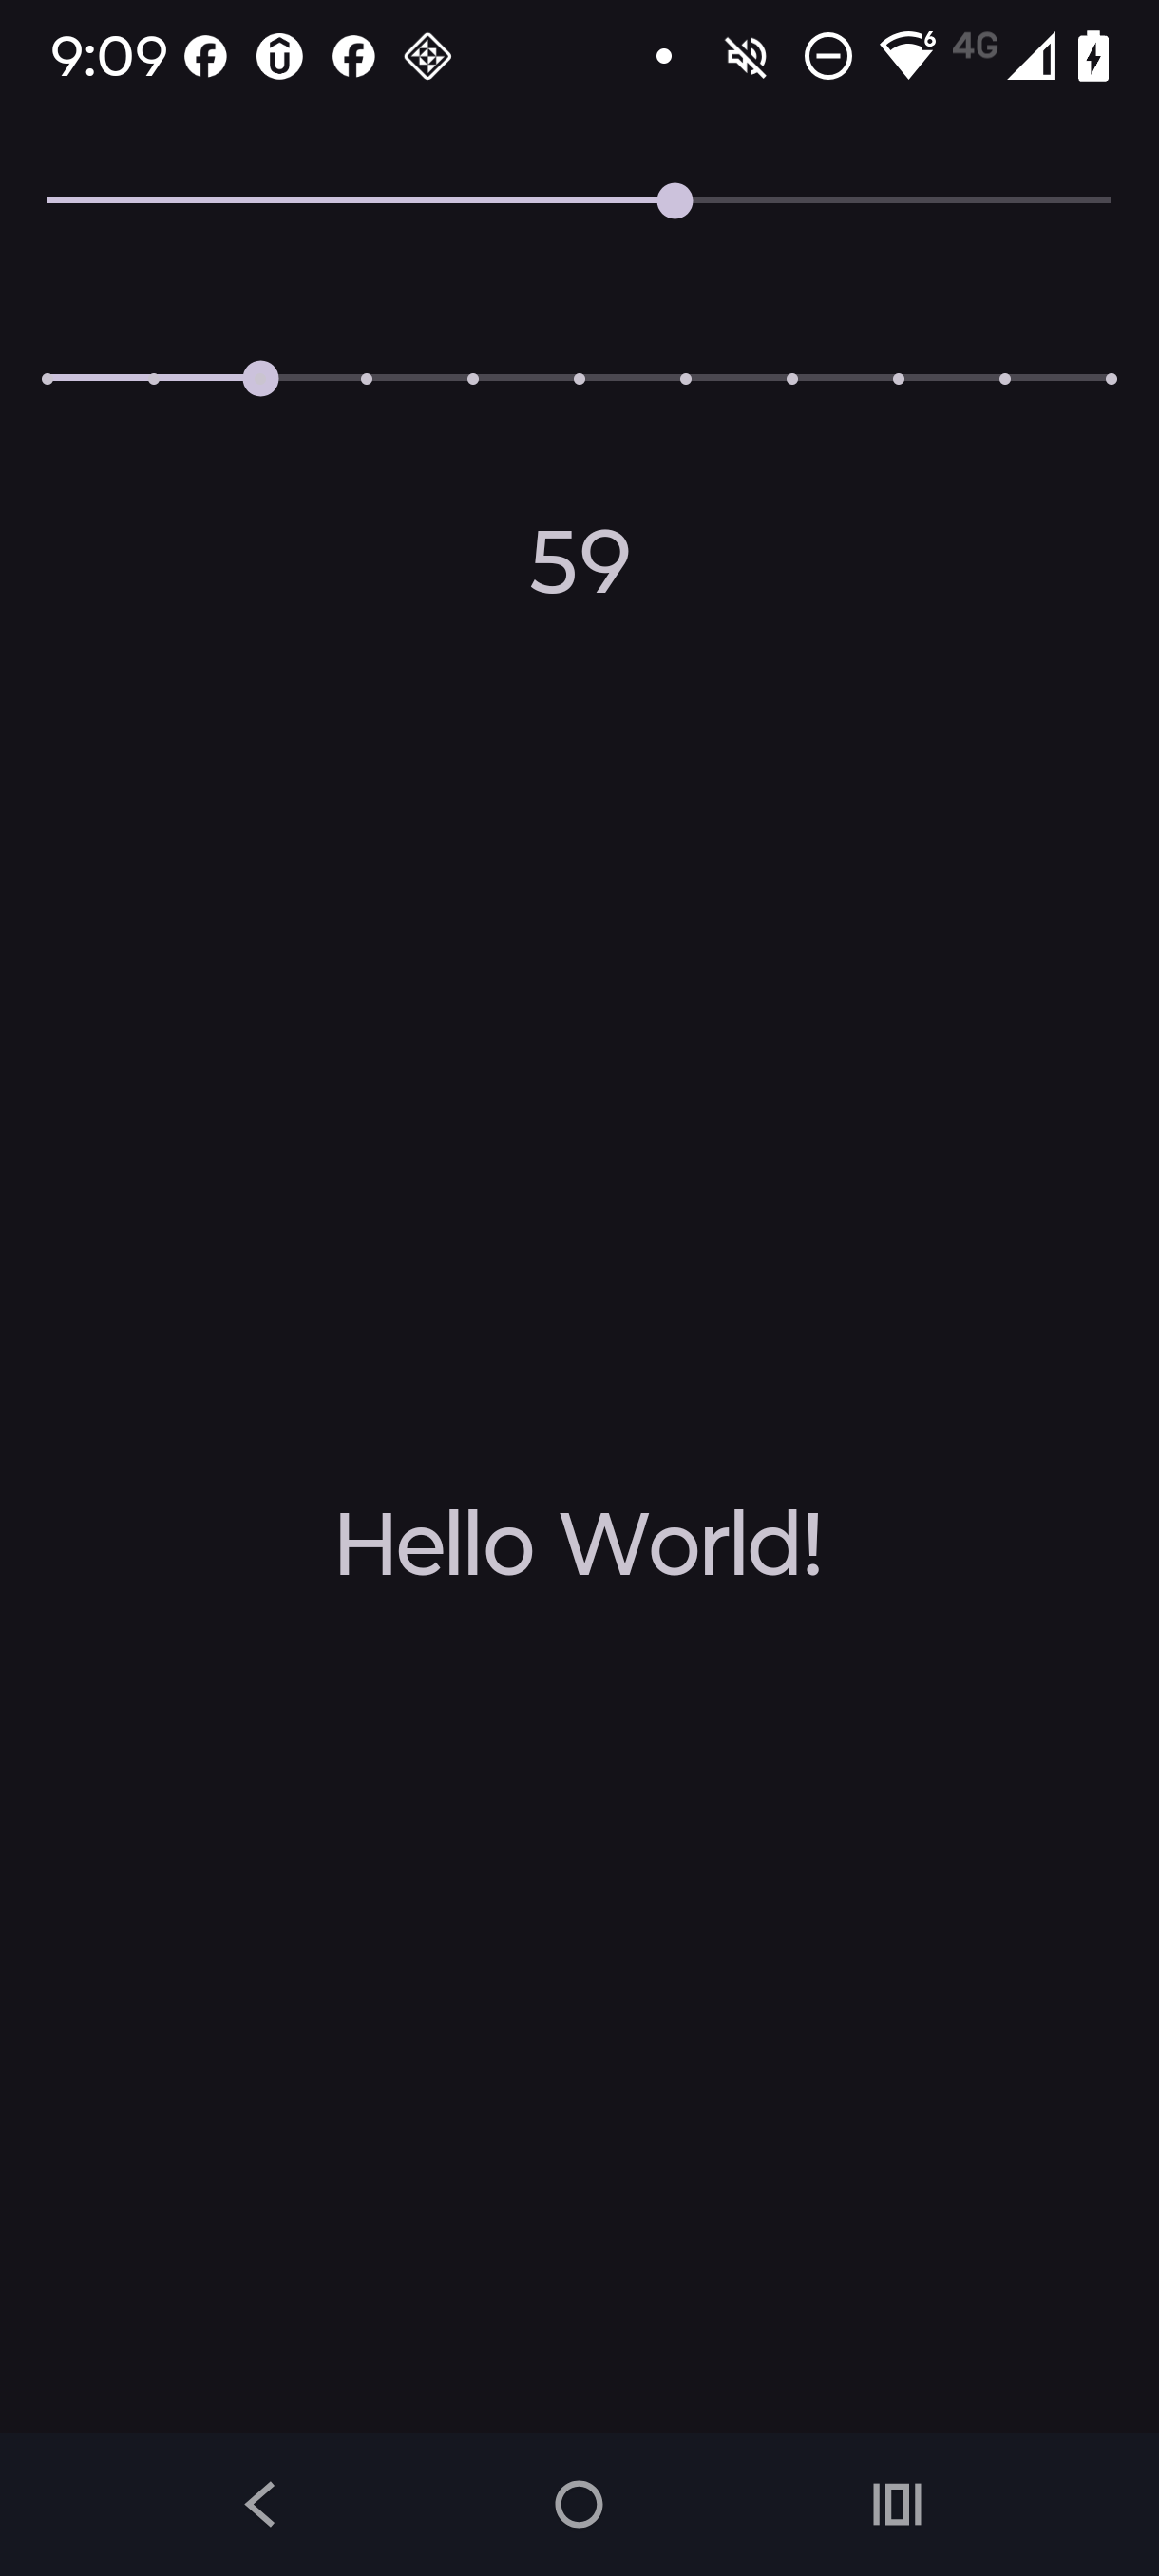
\includegraphics[width=0.98\textwidth]{02_TallerCBTis/figs/Demo08}
\end{center}

\end{columns}

\end{frame}



%\begin{frame}{startActivityForResult y onActivityResult}


\begin{frame}[fragile]
\frametitle{startActivityForResult y onActivityResult}  
\textbf{¿Para qué sirven?}

\begin{itemize}
    \item Permiten iniciar una actividad esperando un resultado de regreso.
    \item Son útiles cuando se necesita que una segunda pantalla devuelva información (por ejemplo, selección de datos o confirmaciones).
\end{itemize}

\vspace{0.4cm}

\textbf{Flujo de funcionamiento:}
\begin{enumerate}
    \item Se inicia la actividad con \texttt{startActivityForResult()}.
    \item La segunda actividad procesa la información.
    \item Se devuelve un resultado mediante \texttt{setResult()}.
    \item La actividad original recibe el resultado en \texttt{onActivityResult()}.
\end{enumerate}


\textbf{Ejemplo en Java:}
\begin{block}{}
\small
\begin{minted}[linenos,fontsize=\tiny]{java}
// Lanzar actividad
Intent intent = new Intent(this, SegundaActivity.class);
startActivityForResult(intent, 1);

// Recibir resultado
@Override
protected void onActivityResult(int requestCode, int resultCode, Intent data) {
    if (requestCode == 1 && resultCode == RESULT_OK) {
        String resultado = data.getStringExtra("dato");
    }
}
\end{minted}
\end{block}

\end{frame}




\begin{frame}[fragile]
\frametitle{Demo 09: Lectura y Escritura de Archivos de Texto}
\begin{columns}
\column{0.80\linewidth}
Del Repositorio Github:
\begin{itemize}
\item Copiar el archivo \textit{MainActivity\_Demo09.java} (dentro del Folder códigosJAVA) al mismo directorio donde esta el MainActivity.java
\item Copiar el archivo \textit{activity\_main\_demo09.xml} (dentro del Folder Carpeta\_layout) al mismo directorio donde esta el activity\_main.xml

%\item Copiar los archivos \textit{cgup.jpg} y \textit{logo\_upv\_2019.png} localizados dentro de la folder \textit{Carpeta\_drawable} en el directorio \textit{res/drawable} del proyecto de AS.
\item Modificar en el archivo \textit{AndroidManifest.xml} la cadena \textit{.MainActivity\_Demo08} por \textit{.MainActivity\_Demo09}.
\item Ir a la linea 22 de archivo del archivo \textit{MainActivity\_Demo09.java}, poner el cursos en la palabra (en Rojo) \textit{documentfile}, presionar la combinación ALT+ENTER, y seleccionar de la lista desplegable la opcion ``Add dependency on ....''. Esto quitará el error y hara los ajustes necesarios. 
\end{itemize}

%\begin{block}{Demo \#09}
%Un App que permite escribir el contenido de un EditText a un archivo y cargar el contenido de cualquier archivo en el EditText
%\end{block}


\column{0.20\linewidth}

\begin{center}
 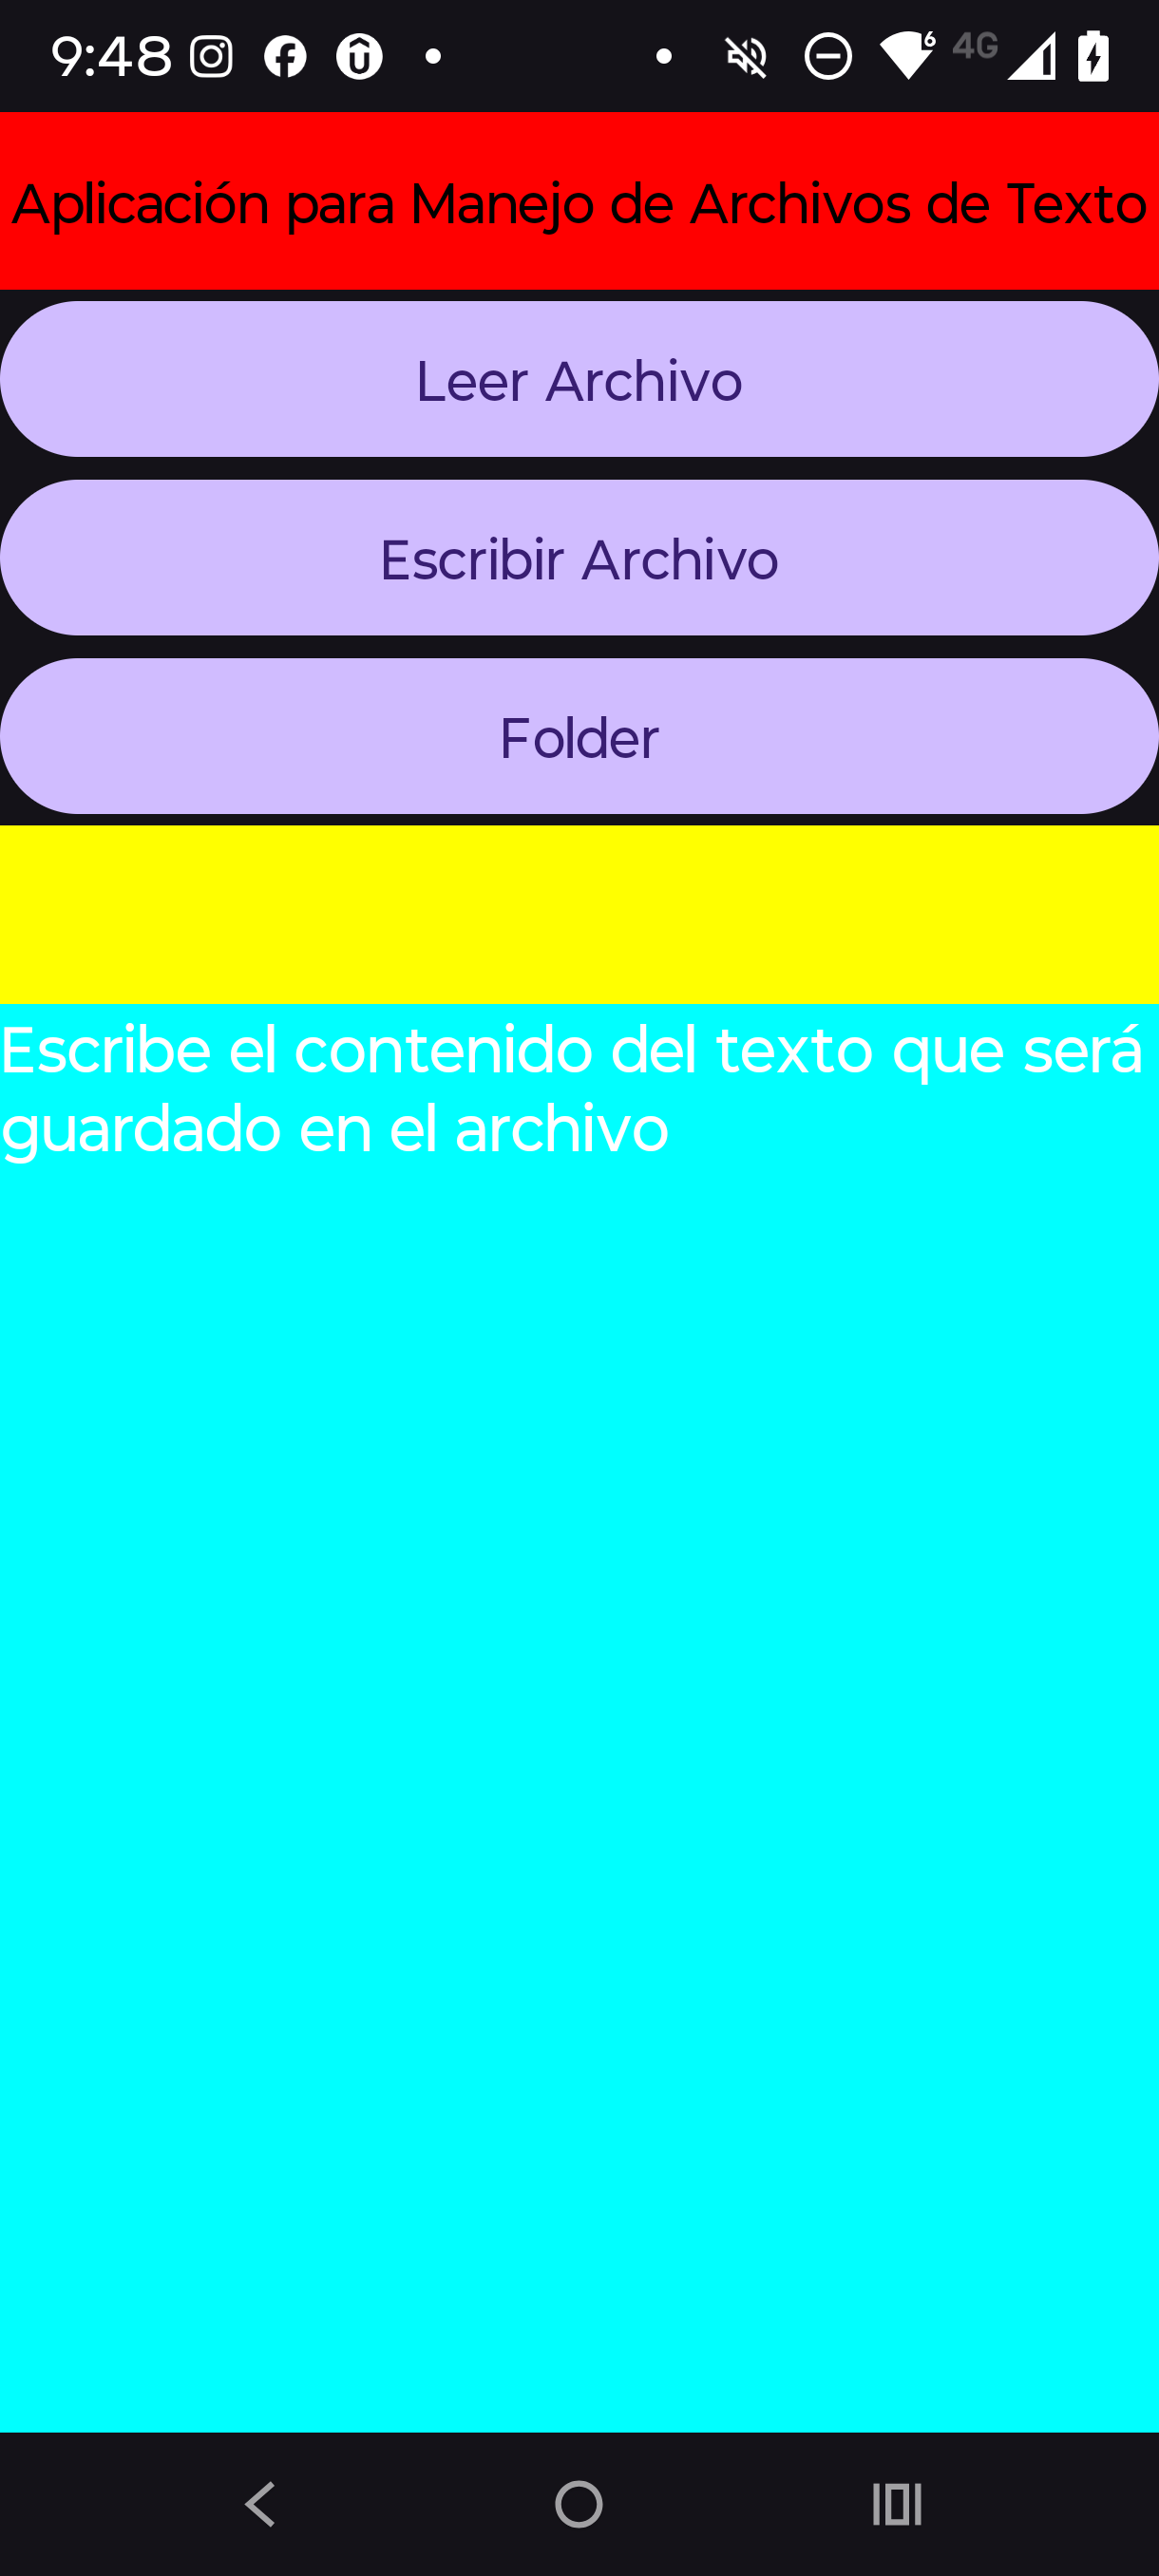
\includegraphics[width=0.98\textwidth]{02_TallerCBTis/figs/Demo09}
\end{center}

\end{columns}

\end{frame}

